\documentclass[10pt]{book}
\usepackage[utf8]{inputenc}
\usepackage[italian]{babel}
\usepackage{multicol}
\usepackage[bookmarks]{hyperref}
\usepackage[a4paper, total={18cm, 25cm}]{geometry}
\usepackage{listings}
\usepackage{graphicx}
\usepackage{makecell}
\usepackage{amssymb}
\graphicspath{ {./img/} }
\usepackage{color}
\definecolor{mygray}{rgb}{0.5,0.5,0.5}
\usepackage{listings}
\lstset{
	language=SQL,
	breaklines=true,
	keywordstyle=\bfseries,
	identifierstyle=\ttfamily,
	commentstyle=\color{mygray},
	morekeywords={database, REFERENCES, SCHEMA, AUTHORIZATION, PROCEDURE, WITH, CHECK, OPTION, FOR, EACH, ROW, DECLARE, BEFORE, AFTER, IF, TO, PRIVILEDGES, COMMIT, WORK, ROLLBACK},
}

\begin{document}
\renewcommand*\contentsname{Indice}
\title{Basi di Dati}
\author{Federico Matteoni}
\date{A.A. 2019/20}
\maketitle
\tableofcontents
\pagebreak
\chapter*{Introduzione}
\paragraph{Obiettivi del corso} Modelli dei dati, linguaggi e sistemi per lo sviluppo di applicazioni che prevedono l'uso di grandi quantità di dati permanenti organizzati in \textbf{basi di dati}.
\paragraph{Testo di Riferimento} \textit{Fondamenti di Basi di Dati}, A. Albano, G. Ghelli e R. Orsini, Zanichelli. Scaricabile liberamente da \texttt{fondamentidibasididati.it}
\paragraph{Terminologia}
\begin{list}{}{}
	\item \textbf{Base di dati}: tecnologia di base, gestione delle attività quotidiane dell'organizzazione e \textbf{tema di questo corso}
	\item Data Warehouse, Data Lake, Big Data, Data Science: termini che hanno a che vedere con l'\textbf{analisi dei dati} e che non rientrano nei temi trattati nel corso.
\end{list}
\chapter{Costruzione di una base di dati}
\paragraph{Cos'è una base di dati?} Una \textbf{base di dati} è un \textbf{insieme organizzato di dati} usati per il supporto allo svolgimento di un'attività (di un ente, azienda, ufficio, persona\ldots)
\paragraph{Qualche esempio}
\begin{center}
\textbf{Materie}\\
	\begin{tabular}{c | c | c}
	\textbf{Titolo} & \textbf{Codice} & \textbf{Syllabus} \\
	\hline
	Basi di Dati & AA024 & Progettazione e interrogazione\ldots \\
	\hline
	Reti di Calcolatori & AA019 & Realizzazione e uso di reti, protocollo TCP\ldots
	\end{tabular}
\end{center}
\begin{center}
\textbf{Corsi}\\
	\begin{tabular}{c | c | c | c}
	\textbf{Materia} & \textbf{AA} & \textbf{Semestre} & \textbf{Titolare} \\
	\hline
	AA024 & 2007 & 1 & Albano \\
	\hline
	AA024 & 2007 & 1 & Ghelli \\
	\hline
	AA019 & 2007 & 1 & Brogi 
	\end{tabular}
\end{center}
\section{Elementi}
\subsection{Figure Coinvolte}
\begin{list}{}{}
	\item \textbf{Committente}
	\begin{list}{}{}
		\item Dirigente
		\item Operatore
	\end{list}
	\item \textbf{Fornitore}
	\begin{list}{}{}
		\item Direttore del progetto
		\item Analista
		\item Progettista del DB
		\item Programmatore di applicazioni che usano il DB
	\end{list}
	\item Manutenzione e messa a punto del DB -- \textbf{Gestione del DBMS}
	\begin{list}{}{}
		\item Amministratore del DBMS
	\end{list}
\end{list}
\subsection{Sistemi Informativi}
\paragraph{Definizione} Un \textbf{sistema informativo} di un'organizzazione è una \textbf{combinazione di risorse, umane e materiali, e di procedure} organizzate per raccolta, archiviazione, elaborazione e scambio \textbf{delle informazioni} necessarie alle attività:
\begin{list}{}{}
	\item \textbf{Operative} (informazioni di servizio)
	\item Programmazione e \textbf{controllo} (informazioni di gestione)
	\item \textbf{Pianificazione} strategica (informazioni di governo)
\end{list}
\pagebreak
\paragraph{Esempi di sistemi informativi}
\begin{list}{}{Un comune}
	\item Gestione servizi demografici (anagrafe, stato civile, servizio elettorale e vaccinale) e della rete viaria
	\item Gestione attività finanziaria secondo la normativa vigente
	\item Gestione del personale per il calcolo della retribuzione in base al tipo di normativa contrattuale
	\item Gestione dei servizi amministrativi e sanitari delle USL
	\item Gestione della cartografia generale e tematica del territorio
\end{list}
\paragraph{Sistema informativo nelle organizzazioni}
\begin{center}
	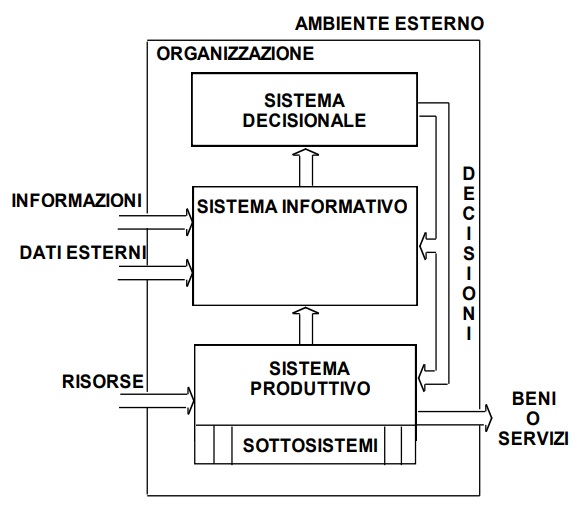
\includegraphics[scale=0.7]{sisinformativoorg.png}
\end{center}
\subsection{Sistemi Informatici}
\paragraph{Sistema Informativo Automatizzato} Quella parte del sistema informativo in cui le informazioni sono raccolte, elaborate, archiviate e scambiate usando un \textbf{sistema informatico}.
\paragraph{Sistema Informatico} Insieme delle tecnologie informatiche e della comunicazione (\textbf{ICT}, Information and Communication Technologies) a supporto delle attività di un'organizzazione.
\paragraph{Terminologia}
\begin{center}
Sistema informativo $\longrightarrow$ Sistema informativo automatizzato\\
Sistema informativo automatizzato $\longrightarrow$ Sistema informatico
\end{center}
\begin{center}
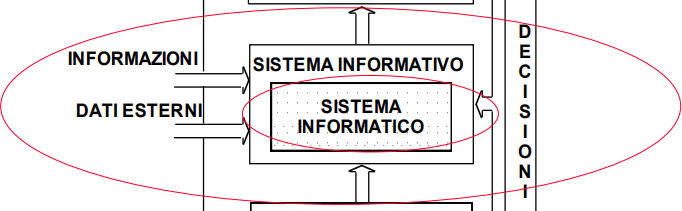
\includegraphics[scale=0.7]{sisinformativoorg2.png}
\end{center}
\pagebreak
\subsection{Classificazione dei sistemi informatici}
\begin{center}
Sistemi Informatici Operativi $\longrightarrow$ Sistemi Informatici Direzionali
\end{center}
\begin{multicols}{2}
\paragraph{Sistemi Informatici Operativi} I dati sono organizzati in DB. Le applicazioni si usano per svolgere le classiche attività strutturate e ripetitive dell'azione nelle aree amministrativa e finanziaria: vendite, risorse umane, produzione\ldots\\
\textbf{Alcune sigle}:
\begin{list}{}{}
	\item \textbf{DP} Data Processing\\\textbf{EDP} Electronic Data Processing
	\item \textbf{TPS} Transaction Processing Systems
\end{list}
\begin{center}
	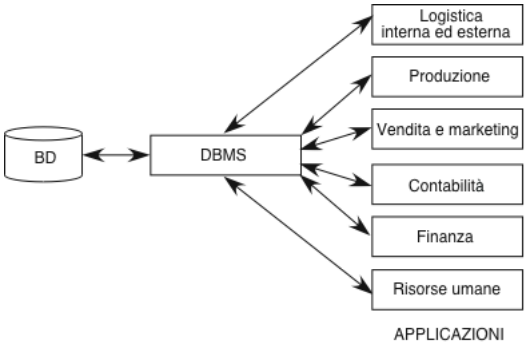
\includegraphics[scale=0.6]{sisinfop.png}
\end{center}
\paragraph{DBMS} Le caratteristiche del DB sono \textbf{garantite da un sistema per la gestione della base di dati} (\textbf{DBMS}, Data Base Management System) che ha il controllo dei dati e li rende accessibili agli utenti autorizzati.
\paragraph{OLTP} \textbf{On-Line Transaction Processing}, modo d'uso principale dei DBMS. Tradizionale elaborazione di transazioni, che realizzano processi operativi per il funzionamento di organizzazioni:
\begin{list}{}{}
	\item Operazioni predefinite e relativamente semplici
	\item Ogni operazione coinvolge \textit{pochi} dati
	\item Dati di dettaglio, aggiornati
\end{list}
\end{multicols}
\begin{multicols}{2}
\paragraph{Sistemi Informatici Direzionali} I dati sono organizzati in data warehouse (DW) e gestiti da un opportuno sistema. Le applicazioni, dette di \textbf{business intelligence}, sono strumenti di supporto ai processi di controllo delle prestazioni aziendali e di decisione manageriale. Terminologia:
\begin{list}{}{}
	\item \textbf{MIS} Management Information Systems
	\item \textbf{DSS} Decision Support Systems, data-based o model-based
	\item \textbf{EIS} Executive Information System
\end{list}
\begin{center}
	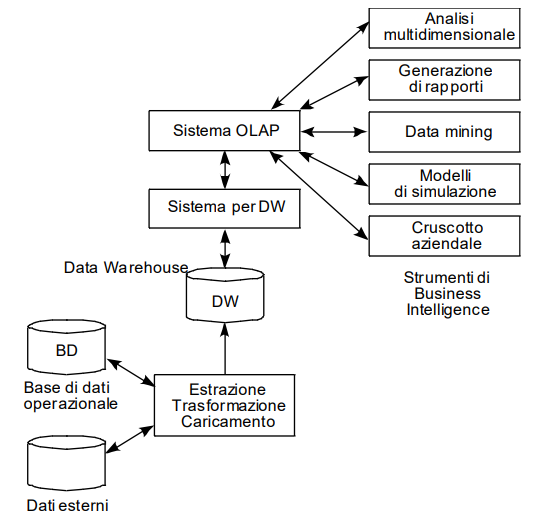
\includegraphics[scale=0.6]{sisinfdir.png}
\end{center}
\columnbreak
\paragraph{OLAP} \textbf{On-Line Analytical Processing} modo d'uso principale dei DW. Analisi dei dati di supporto alle decisioni:
\begin{list}{}{}
	\item Operazioni complesse e casuali
	\item Ogni operazione può coinvolgere \textit{molti} dati
	\item Dati aggregati, storici, anche non attualissimi
\end{list}
\end{multicols}
\pagebreak
\paragraph{Differenze tra OLTP e OLAP}
\begin{center}
	\begin{tabular}{r | l | l}
	 & \makecell{\textbf{OLTP}} & \makecell{\textbf{OLAP}} \\
	\textbf{Scopi} & Supporto operatività & Supporto decisioni \\
	\textbf{Utenti} & Molti, esecutivi & Pochi, dirigenti e analisti \\
	\textbf{Dati} & Analitici, relazionali & Sintetici, multidimensionali \\
	\textbf{Usi} & Noti a priori & Poco prevedibili \\
	\textbf{Quantità di dati per attività} & Bassa (decine) & Alta (milioni) \\
	\textbf{Orientamento} & Applicazione & Soggetto \\
	\textbf{Aggiornamenti} & Frequenti & Rari \\
	\textbf{Visione dei dati} & Corrente & Storica \\
	\textbf{Ottimizzati per} & Transazioni & Analisi
	\end{tabular}
\end{center}
\subsection{Requisiti per l'Analisi dei Dati}
\paragraph{Aggregati} Non interessa \textbf{un} dato, ma la \textbf{somma}, la \textbf{media}, il \textbf{minimo}/\textbf{massimo} di una misura\ldots
\paragraph{Multidimensionale} Interessa \textbf{incrociare le informazioni}, per analizzarle da punti di vista diversi e valutare i risultati del business per intervenire sui problemi critici o per cogliere nuove opportunità
\paragraph{Diversi livelli di dettaglio} Per esempio, una volta scoperto un calo delle vendite in un determinato periodo in una specifica regione, si passa ad un'analisi dettagliata nell'area di interesse per cercare di scoprirne le cause (dimensioni con \textbf{gerarchie})
\subsection{Big Data}
\paragraph{Ampio} Big data è un termine ampio riferito a situazioni in cui l'approccio "schema-first" tipico di DB e DW risulta troppo restrittivo o troppo lento.
\paragraph{3 V} Volume, Varietà, Velocità
\paragraph{} I Big Data sono in genere associati a sistemi NoSQL, machine learning e approcci Data Lake.
\section{DBMS}
Un \textbf{DBMS} è un sistema (\textbf{software}) in grado di \textbf{gestire collezioni di dati} che siano, tra le altre cose:
\begin{list}{}{}
	\item \textbf{Grandi}
	\item \textbf{Persistenti}, con un periodo di vita indipendente dalle singole esecuzioni dei programmi che le utilizzano
	\item \textbf{Condivise}, usate da applicazioni diverse
\end{list}
garantendo \textbf{affidabilità} (resistenza a malfunzionamenti hardware e software-recovery) e \textbf{privacy} (con una disciplina e un controllo degli accessi).\\
Come ogni altro software, un DBMS deve essere \textbf{efficiente} (usare al meglio le risorse di spazio e tempo del sistema) ed \textbf{efficace} (rendere produttive le attività degli utilizzatori).\\
Un DBMS offre opportuni linguaggi per:
\begin{list}{}{}
	\item \textbf{Definire lo schema} di un DB, che va definito prima di creare dati
	\item \textbf{Scegliere le strutture dati} per la memorizzazione
	\item Memorizzare i dati \textbf{rispettando i vincoli} definiti nello schema
	\item Recuperare e modificare i dati, interattivamente (\textbf{query language}, linguaggio di interrogazione) o da programmi
\end{list}
\subsection{Dati}
I dati permanenti contenuti in un DB sono divisi in due categorie:
\begin{list}{}{}
	\item \textbf{Metadati}\\
	Descrivono dati sullo schema dei dati, utenti autorizzati, applicazioni, parametri quantitativi\ldots\\
	I metadati sono descritti da uno schema usando il modello dei dati usato dal DBMS e sono interrogabili con le stesse modalità previste dai dati
	\item \textbf{Dati}\\
	Rappresentazioni di certi fatti conformi alle definizioni dello schema. Hanno le seguenti caratteristiche:
	\begin{list}{}{}
		\item Organizzati in \textbf{insiemi strutturati e omogenei}, fra i quali sono definite delle \textbf{relazioni}. La struttura dei dati e le relazioni sono \textbf{descritte nello schema} usando i meccanismi di astrazione del modello dei dati del DBMS.
		\item Sono \textbf{molti}, sia in assoluto che rispetto ai metadati, e non possono essere gestiti in memoria temporanea
		\item Sono \textbf{accessibili mediante transazioni}, \textbf{unità di lavoro atomiche} che \textbf{non possono avere effetti parziali}
		\item Sono \textbf{protetti} sia \textbf{da accesso da parte di utenti non autorizzati}, sia \textbf{da corruzione dovuta a malfunzionamenti} hardware o software
		\item Sono \textbf{utilizzabili contemporaneamente da utenti diversi}
	\end{list}
\end{list}
Il \textbf{modello relazionale dei dati} è il più diffuso fra i DBMS commerciali. Il \textbf{meccanismo di astrazione} fondamentale è la \textbf{relazione} (\textbf{tabella}), sostanzialmente un insieme di record dai campi elementari.\\
Lo schema di una relazione ne definisce il nome e ne descrive la struttura dei possibili elementi della relazione (insieme di attributi con il loro tipo)
\paragraph{Esempio}
\begin{list}{}{}
	\item \textbf{Definizione del DB}
	\begin{lstlisting}
create database EsempioEsame
	\end{lstlisting}
	\item \textbf{Definizione schema}
	\begin{lstlisting}
create table Esami(Materia char(5), Candidato char(8), Voto int, Lode char(1),
Data char(6))
	\end{lstlisting}
	\item \textbf{Inserzione dati}
	\begin{lstlisting}
insert into Esami values ('BDSI1', '080709', 30 'S', '070900')
	\end{lstlisting}
	\item \textbf{Interrogazione}
	\begin{lstlisting}
select Candidato from Esami where Materia = "BDSI1" and Voto = 30
	> Candidato
	> 080709
	\end{lstlisting}
\end{list}
\pagebreak
\subsection{DDL}
\paragraph{Data Definition Language} Linguaggio per la definizione della base di dati.\\
Utile distinguere tre diversi livelli di descrizione dei dati (\textbf{schemi}):
\begin{multicols}{2}
\begin{list}{}{}
	\item Livello di \textbf{vista logica}
	\item Livello \textbf{logico}
	\item Livello \textbf{fisico}
\end{list}
\begin{center}
	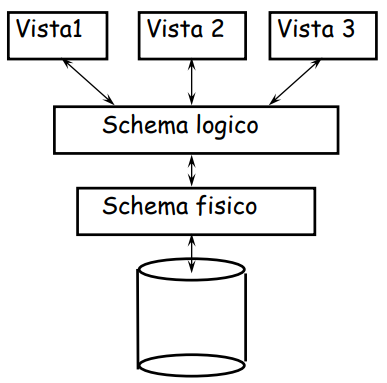
\includegraphics[scale=0.5]{livellidescrdati.png}
\end{center}
\end{multicols}
\paragraph{Livello Logico} Descrive la struttura degli insiemi di dati e delle relazioni fra loro, secondo un certo modello dei dati, senza nessun riferimento alla loro organizzazione fisica nella memoria permanente.\\
Esempi:
\begin{lstlisting}
Studenti(Matricola char(8), Nome char(20), Login char(8), Anno int, Reddito float)
Corsi(IdeC char(8), Titolo char(20), Credito int)
Esami(Matricola char(8), IdeC char(8), Voto int)
\end{lstlisting}
\paragraph{Livello Fisico} Descrive come vanno organizzati fisicamente i dati nelle memorie permanenti e quali strutture dati ausiliarie prevedere per facilitarne l'uso (schema fisico o interno).\\
Esempi: relazioni Studenti e Esami organizzate in modo seriale, Corsi organizzata sequenziale con indice, indice su Matricola.
\paragraph{Vista Logica} Descrive come deve \textbf{apparire la struttura} del DB ad una certa applicazione (\textbf{schema esterno} o \textbf{vista}). Esempio:
\begin{lstlisting}
InfCorsi (IdeC char(8), Titolo char(20), NumEsami int)
\end{lstlisting}
Nell'organizzazione di una banca, lo \textbf{schema logico} conterrà tutte le tabelle e i dati relativi ai conti correnti, ma anche al personale. Lo schema logico conserva \textbf{tutte le informazioni} della banca. Nello \textbf{schema esterno} ogni correntista potrà \textbf{accedere solo ad alcune informazioni} di suo interesse: quelle del proprio conto corrente.
\paragraph{Indipendenza} L'approccio con tre livelli è stato proposto per garantire le proprietà di indipendenza logica e fisica dei dati, fra gli obiettivi più importanti dei DBMS.
\begin{list}{}{}
	\item \textbf{Indipendenza fisica}: i programmi applicativi non devono essere modificati in seguito a modifiche dell'organizzazione fisica dei dati
	\item \textbf{Indipendenza logica}: i programmi applicativi non devono essere modificati in seguito a modifiche dello schema logico
\end{list}
\subsection{DML}
\paragraph{Data Manipulation Language} Linguaggio per l'uso dei dati.\\
Un DBMS deve prevedere più modalità d'uso per soddisfare esigenze di diverse categorie d'utenti: GUI per accedere ai dati, linguaggio di interrogazione per i non programmatori, linguaggio di programmazione per chi sviluppa le applicazioni, linguaggio di sviluppo per le interfacce delle applicazioni.\\
Linguaggi vari e interfacce diverse:
\begin{list}{}{}
	\item Linguaggi testuali interattivi, SQL
	\item Comandi (come quelli del linguaggi interattivo) immersi in un linguaggio ospite, come il C
	\item Comandi (come quelli del linguaggi interattivo) immersi in un linguaggio ad hoc (come PL/SQL) con anche altre funzionalità (come grafici e stampe strutturate)
	\item Interfacce amichevoli
\end{list}
\subsection{Schemi e Istanze}
\paragraph{Schema} Descrive la \textbf{struttura dei dati}, sostanzialmente invariante nel tempo: le "classi", intestazione delle tabelle
\paragraph{Istanza} \textbf{Valori attuali} dei dati che possono cambiare anche molto rapidamente: gli "oggetti", il corpo di ciascuna tabella
\subsection{Meccanismi per il controllo dei dati}
Caratteristica molto importante dei DBMS è il tipo di meccanismi usati per garantire le seguenti proprietà
\begin{list}{}{}
	\item \textbf{Integrità}: mantenimento delle proprietà specificate nello schema
	\item \textbf{Sicurezza}: protezione da usi non autorizzati
	\item \textbf{Affidabilità}: protezione da malfunzionamenti e interferenze dovute all'accesso concorrente di più utenti
\end{list}
\subsection{Transazioni}
\paragraph{Definizione} Una \textbf{transazione} è una \textbf{sequenza di azioni di lettura/scrittura in memoria permanente e di elaborazione dati in memoria temporanea}, con le seguenti proprietà:
\begin{list}{}{}
	\item \textbf{Atomicità}: le transazioni che terminano prematuramente (\textbf{aborted transactions}) sono \textbf{trattate dal sistema come se non fossero mai iniziate}. Eventuali effetti sul DB sono \textbf{annullati}.
	\item \textbf{Serializzabilità}: esecuzioni concorrenti di più transazioni danno come effetto quello di una esecuzione seriale
	\item \textbf{Persistenza}: le \textbf{modifiche} sul DB di una transazione terminata normalmente sono \textbf{permanenti}, cioè \textbf{non alterabili da malfunzionamenti}
\end{list}
\section{Progettazione}
\paragraph{Progettare} Progettare un DB significa \textbf{progettare la struttura dei dati e delle applicazioni}. La progettazione dei dati è l'attività più importante e per progettare al meglio i dati è necessario che essi siano un \textbf{modello fedele del dominio} in esame. Per questo ora parleremo della \textbf{modellazione}.
\subsection{Modellazione}
\paragraph{Definizione} Un \textbf{modello astratto} è la \textbf{rappresentazione formale di idee e conoscenze relative ad un fenomeno}.\\
Aspetti di un modello:
\begin{list}{}{}
	\item Il \textbf{modello} è la \textbf{rappresentazione di certi fatti}.
	\item La \textbf{rappresentazione} è \textbf{data con un linguaggio formale}.
	\item Il \textbf{modello} è \textbf{il risultato di un processo di interpretazione}, guidato dalle idee e conoscenze possedute dal soggetto che interpreta.
\end{list}
\textbf{La stessa realtà può utilmente essere modellata in modi diversi e a diversi livelli di astrazione}.
\begin{center}
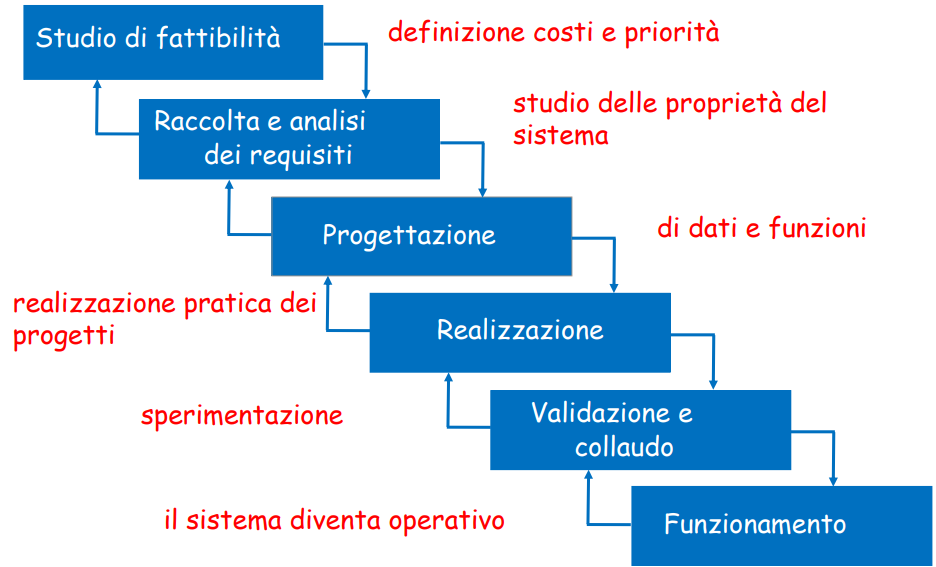
\includegraphics[scale=0.7]{modellaz.png}
\end{center}
\paragraph{Metodologia di progetto} Per garantire prodotti di buona qualità è opportuno seguire una metodologia di progetto, con:
\begin{list}{}{}
	\item Articolazione delle attività in fasi (\textbf{decomposizione})
	\item Criteri di scelta (\textbf{strategie})
	\item \textbf{Modelli} da rappresentare
	\item \textbf{Generalità} rispetto al problema in esame e agli strumenti a disposizione
	\item \textbf{Qualità} del prodotto
	\item \textbf{Facilità d'uso}
\end{list}
\paragraph{Progettazione della base di dati} Suddivisa nelle seguenti fasi:
\begin{enumerate}
	\item \textbf{Analisi} dei requisiti
	\item Progettazione \textbf{concettuale}
	\item Progettazione \textbf{logica}
	\item Progettazione \textbf{fisica}
\end{enumerate}
Ciascuna fase è incentrata sulla modellazione, che discuteremo quindi con riferimento alla problematica della progettazione del DB.
\paragraph{Modello dei dati} Insieme di costrutti utilizzati per organizzare i dati di interesse e descriverne la dinamica. Il componente fondamentale è l'insieme dei \textbf{meccanismi di strutturazione} (o \textbf{costruttori di tipo}). Come nei linguaggi di programmazione, esistono meccanismi che permettono di definire nuovi tipi, così \textbf{ogni modello dei dati prevede alcuni costruttori}: per esempio, il \textbf{modello relazionale prevede il costruttore \textit{relazione}}, che permette di definire insiemi di record omogenei.
\pagebreak
\subsection{Aspetti del problema}
\subsubsection{Aspetto ontologico} Quale conoscenza del dominio del discorso si rappresenta? Ontologico cioè studio di ciò che si suppone esista nell'universo del discorso e che sia quindi necessario modellare.
\begin{list}{}{Cosa si modella:}
	\item \textbf{Conoscenza concreta}: i fatti
	\item \textbf{Conoscenza astratta}: la struttura e i vincoli sulla conoscenza concreta
	\item \textbf{Conoscenza procedurale}, comunicazioni: le operazioni base, le operazioni degli utenti, come si comunicherà con il sistema informatico
\end{list}
Ci concentreremo sulla conoscenza concreta e astratta.
\subsubsection{Aspetto logico} Con quali meccanismi di astrazione si modella? Il modello dei dati a oggetti.
\paragraph{Modello dei dati} Insieme dei meccanismi di astrazione per descrivere la struttura della conoscenza concreta.\\
\textbf{Schema}: descrizione della \textbf{struttura della conoscenza concreta} e dei \textbf{vincoli di integrità} usando un particolare modello dei dati.\\\\
Useremo come notazione grafica una \textbf{variante} dei diagrammi a oggetti (o diagrammi Entità-Relazione, diagrammi ER). Nozioni fondamentali: oggetto, tipo di oggetto, classe, ereditarietà, gerarchia fra tipi e gerarchia fra classi.
\subsubsection{Aspetto linguistico} Con quale linguaggio formale si definisce un modello?
\subsubsection{Aspetto pragmatico} Come si procede per costruire un modello? Metodologia da seguire nel processo di modellazione, cioè l'insieme di regole finalizzate alla costruzione del modello informatico.
\subsection{Conoscenza concreta}
La conoscenza concreta riguarda i fatti specifici che si vogliono rappresentare:
\begin{list}{}{}
	\item \textbf{Entità}, sono \textbf{ciò di cui interessa rappresentare alcuni fatti o proprietà}. Ad esempio: una descrizione bibliografica di un libro, un libro, un documento, un prestito, un utente della biblioteca\ldots\\
	Le \textbf{proprietà} sono \textbf{fatti che interessano solo in quanto descrivono caratteristiche di determinate entità}. Ad esempio un indirizzo interessa perché è l'indirizzo di un utente. Hanno delle classificazioni:
	\begin{list}{}{}
		\item Primitiva/strutturata
		\item Obbligatoria/opzionale
		\item Univoca/multivalore
		\item Costante/variabile
		\item Calcolata/non calcolata
	\end{list}
	Una proprietà è una coppia attributo-valore di un certo tipo. Ogni entità appartiene ad un \textbf{tipo} che ne specifica la natura. Ogni proprietà ha associato un \textbf{dominio}, l'insieme dei possibili valori.\\
	Una proprietà è \textbf{atomica} se il suo valore non è scomponibile, altrimenti è \textbf{strutturata}. Inoltre è \textbf{univoca} se ha valore unico, altrimenti è \textbf{multivalore}, e \textbf{totale} (obbligatoria) se ogni entità dell'universo in esame ha per essa un valore specificato, altrimenti è detta \textbf{parziale} (opzionale)\\\\
	Certi fatti possono essere interpretati come proprietà in certi contesti e come entità in altri. Ad esempio, una \texttt{DescrizioniBibliografiche} con attributi \texttt{autori}, \texttt{titolo}, \texttt{editore}\ldots, \textbf{oppure} un \texttt{Autori} con attributi \texttt{nome}, \texttt{nazionalità}\ldots e \texttt{Editori} con \texttt{nome}, \texttt{indirizzo}\ldots
	\item \textbf{Collezioni} variabili nel tempo di entità omogenee. Ad esempio, la collezione di tutti gli utenti della biblioteca.
	\item \textbf{Associazioni} fra entità
\end{list}
\subsection{Modellazione ad oggetti}
\paragraph{Oggetti} Ad ogni entità del dominio corrisponde un oggetto del modello. Un \textbf{oggetto} è un'\textbf{entità software con stato, comportamento ed identità} che modella un'entità dell'universo.
\begin{list}{}{}
	\item \textbf{Stato} modellato da un insieme di costanti o variabili con valori di qualsiasi complessità
	\item \textbf{Comportamento} dato da un insieme di procedure locali chiamate \textbf{metodi}, che modellano le operazioni di base che riguardano l'oggetto e le proprietà derivabili da altre.
	\item Un oggetto può rispondere a dai \textbf{messaggi}, restituendo valori memorizzati nello stato o calcolati con una procedura locale.
\end{list}
\paragraph{Classe} \textbf{Insieme di oggetti dello stesso tipo}, modificabile con operatori per includere o estrarre elementi dall'insieme. Può essere specificata a diversi livelli.
\begin{center}
	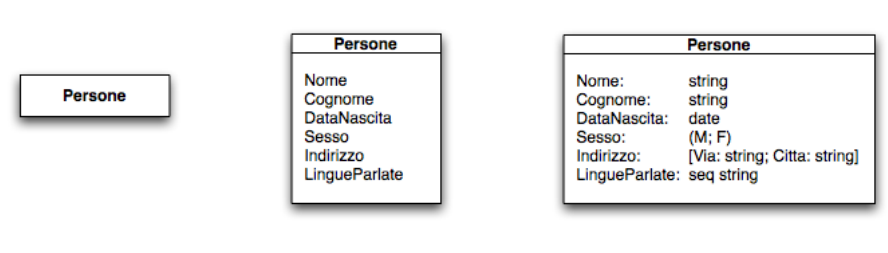
\includegraphics[scale=0.75]{classspec.png}
\end{center}
\paragraph{Tipo oggetto} Il primo passo nella costruzione di un modello consiste nella classificazione delle entità del dominio con la definizione dei tipi degli oggetti che la rappresentano.\\
Un \textbf{tipo oggetto definisce l'insieme dei messaggi} (\textbf{interfaccia}) \textbf{a cui può rispondere un insieme di possibili oggetti}. I nomi dei messaggi sono detti anche attributi degli oggetti.\\
Nei diagrammi ER i tipi oggetti non si rappresentano, perché l'attenzione è sulle collezioni e sulle associazioni. Tuttavia, la rappresentazione grafica di una collezione indica anche gli attributi del tipo oggetto associato.
\paragraph{Associazioni} Un'\textbf{istanza di associazione} è un \textbf{fatto che correla due o più entità}, stabilendo un legame  logico fra loro. Ad esempio, l'utente Tizio ha in prestito una copia della Divina Commedia.\\
Un'associazione \texttt{R(X, Y)} fra due collezioni di entità \texttt{X} e \texttt{Y} è un \textbf{insieme di istanze di associazione} tra elementi di \texttt{X} e di \texttt{Y} che \textbf{varia in generale nel tempo}.\\
Il prodotto cartesiano \texttt{X $\times$ Y} è il dominio dell'associazione.\\
Un esempio:
\begin{center}
	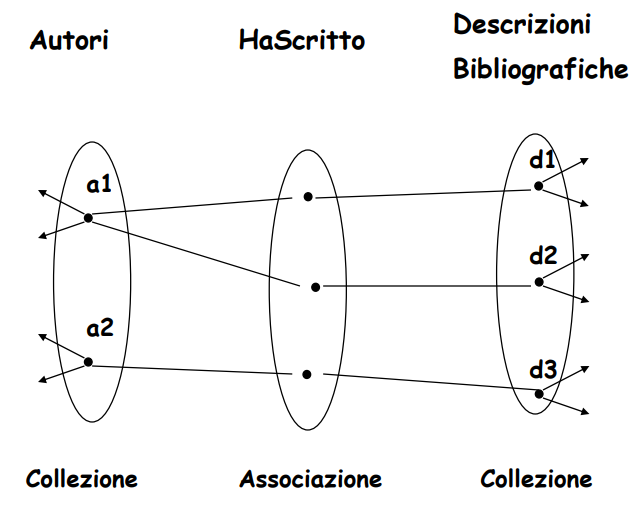
\includegraphics[scale=0.6]{associazioni.png}
\end{center}
\pagebreak
Un associazione è \textbf{caratterizzata da due proprietà strutturali}: \textbf{molteplicità} e \textbf{totalità}.
\subparagraph{Vincolo di univocità} Un'associazione \texttt{R(X, Y)} è \textbf{univoca rispetto a \texttt{X}} se $\forall$\texttt{x} $\in$ \texttt{X} $\exists$ al più un elemento di \texttt{Y} associato ad \texttt{x}.\\
Se non vale questo vincolo, l'associazione è \textbf{multivalore rispetto ad \texttt{X}}.\\\\
\textbf{Cardinalità} dell'associazione:
\begin{list}{}{}
	\item \texttt{R(X, Y)} è \texttt{1:N} se è multivalore su \texttt{X} ed univoca su \texttt{Y}
	\item \texttt{R(X, Y)} è \texttt{N:1} se è univoca su \texttt{X} e multivalore su \texttt{Y}
	\item \texttt{R(X, Y)} è \texttt{N:M} se è multivalore su \texttt{X} e multivalore  su \texttt{Y}
	\item \texttt{R(X, Y)} è \texttt{1:1} se è univoca su \texttt{X} ed univoca su \texttt{Y}
\end{list}
Qualche esempio:
\begin{list}{}{}
	\item \texttt{Frequenta(Studenti, Corsi)} ha cardinalità \texttt{N:M}
	\item \texttt{Insegna(Professori, Corsi)} ha cardinalità \texttt{1:N}
	\item \texttt{SuperatoDa(Esami, Studenti)} ha cardinalità \texttt{N:1}
	\item \texttt{Dirige(Professori, Dipartimenti)} ha cardinalità \texttt{1:1}
\end{list}
\subparagraph{Vincolo di totalità} Un associazione \texttt{R(X, Y)} è \textbf{totale} (o surgettiva) su \texttt{X} se $\forall$ \texttt{x} $\in$ \texttt{X} $\exists$ almeno un elemento di \texttt{Y} associato ad \texttt{x}.\\
Se non vale questo vincolo, l'associazione è \textbf{parziale rispetto a \texttt{X}}.\\
Ad esempio, \texttt{Insegna(Professori, Corsi)} è totale su \texttt{Corsi} perché non può esistere un corso senza il corrispondente docente.
\paragraph{Rappresentazione} Un'associazione si rappresenta con una linea che collega le classi che rappresentano le due collezioni. La linea è etichettata con il nome dell'associazione, di solito scelto utilizzando un predicato.\\
L'univocità dell'associazione rispetto ad una classe si rappresenta disegnando una freccia singola sulla linea che esce dalla classe ed entra nella destinazione. L'assenza di tale vincolo è indicata da una freccia doppia.\\
Similmente, la parzialità è rappresentata da un taglio vicino alla freccia, mentre la totalità è rappresentata dall'assenza del taglio.
\begin{center}
	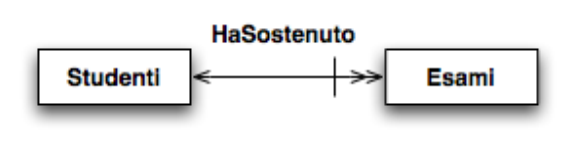
\includegraphics[scale=0.5]{assocesemp.png}\\
	Ogni esame riguarda uno ed un solo studente\\
	Parzialità e assenza di univocità sugli esami\\
	superati da uno studente.\\
	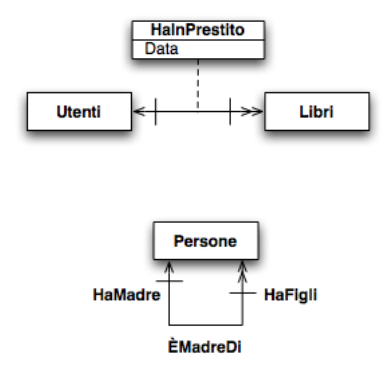
\includegraphics[scale=0.65]{assocesemp2.png}\\
	Possono avere proprietà ed essere ricorsive.
\end{center}
\pagebreak
\subsection{Sottoclassi}
\begin{center}
	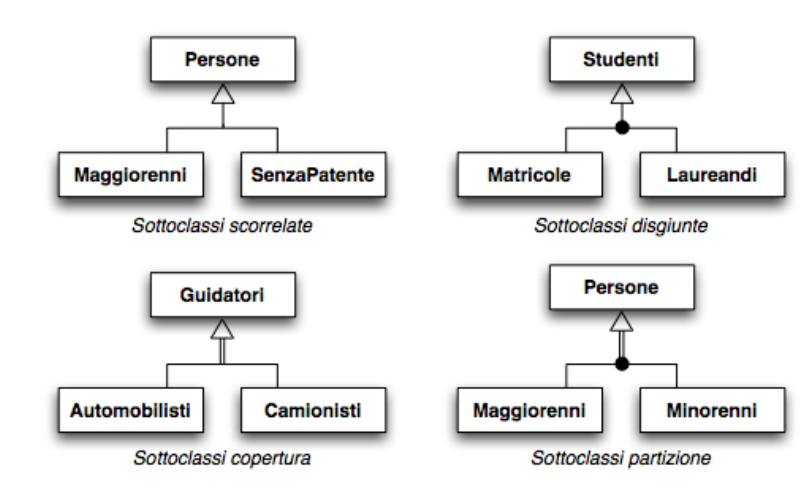
\includegraphics[scale=0.5]{sottoclassi.png}
\end{center}
\paragraph{Vincoli}
\begin{list}{}{}
	\item \textbf{Vincolo intensionale}: C sottoclasse di C' $\Rightarrow$ tipo degli elementi di C è sottotipo del tipo degli elementi di C'
	\item \textbf{Vincolo estensionale}: C sottoclasse di C' $\Rightarrow$ gli elementi di C sono un sottoinsieme degli elementi di C'
	\item \textbf{Disgiunzione}: ogni coppia di sottoclassi è disgiunta, priva di elementi comuni (pallino nero) \textbf{sottoclassi disgiunte})
	\item \textbf{Copertura}: l'unione degli elementi delle sottoclassi coincide con l'insieme degli elementi della superclasse (freccia con doppia asta) (\textbf{sottoclassi copertura})
\end{list}
\subsection{Un esempio elaborato}
\begin{center}
	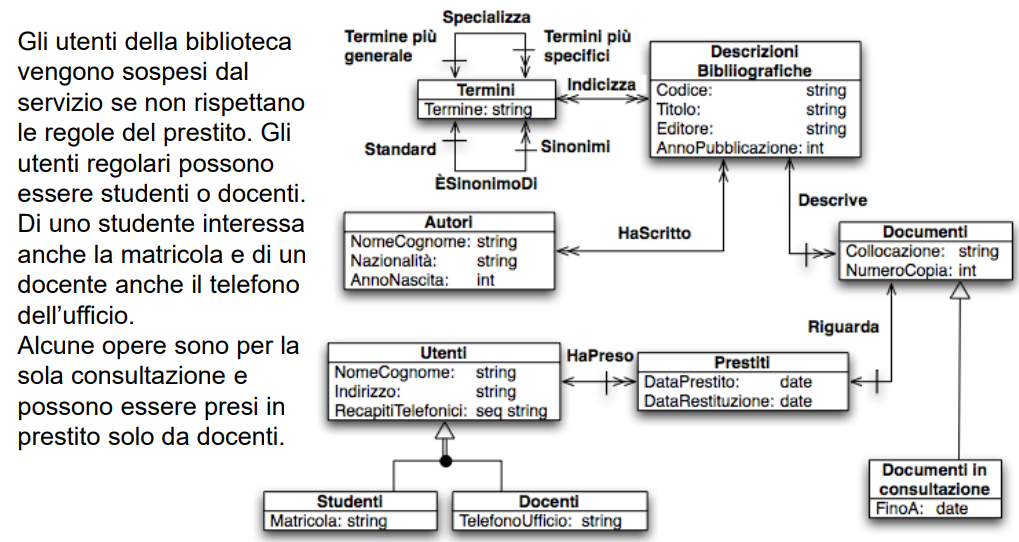
\includegraphics[scale=0.65]{esempioelaborato.png}
\end{center}
\pagebreak
\subsection{Conoscenza astratta}
La conoscenza astratta riguarda i \textbf{fatti generali che descrivono}
\begin{list}{}{}
	\item la \textbf{struttura della conoscenza concreta}, come collezioni, tipi entità, associazioni\ldots
	\item le \textbf{restrizioni sui valori} possibili della conoscenza concreta e sui modi in cui essi possono evolvere nel tempo (\textbf{vincoli d'integrità}, statici e dinamici)
	\item le \textbf{regole per derivare fatti nuovi} da altri noti
\end{list}
\paragraph{Vincoli} Possono essere descritti in \textbf{modo dichiarativo} (da preferire), con formule di calcolo dei predicati, oppure mediante controlli da eseguire nelle operazioni.
\begin{center}
	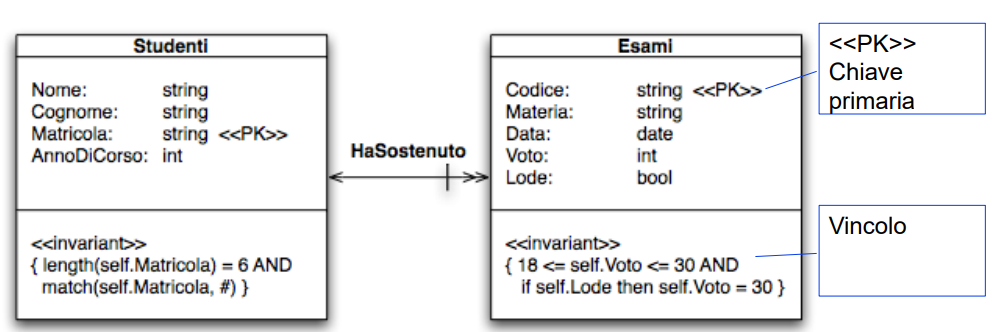
\includegraphics[scale=0.6]{vincoli.png}
\end{center}
\section{Costruzione}
\begin{enumerate}
	\item Analisi dei requisiti $\rightarrow$ specifica dei requisiti, schemi di settore
	\item Progettazione
	\begin{list}{-}{}
		\item Progettazione \textbf{concettuale} ($\rightarrow$ schema concettuale), \textbf{logica} ($\rightarrow$ schema logico), \textbf{fisica} ($\rightarrow$ schema fisico) dei dati
		\item Progettazione delle applicazioni
	\end{list}
	\item Realizzazione
\end{enumerate}
Spesso consideriamo l'analisi dei requisiti come parte della progettazione.
\subsection{Analisi dei requisiti}
\textbf{Analizza il sistema} esistente e \textbf{raccoglie requisiti informali}. Dopodiché \textbf{elimina le ambiguità} e la disuniformità, \textbf{raggruppando frasi relative a diverse categorie} di dati, vincoli e operazioni.\\
Costruisce un \textbf{glossario}, \textbf{disegna lo schema} di settore, \textbf{specifica le operazioni} e \textbf{verifica la coerenza tra operazioni e dati}.
\paragraph{Documentazione descrittiva} In generale, il linguaggio naturale è pieno di ambiguità e fraintendimenti, che bisogna evitare per quanto possibile. Come prima approssimazione si può seguire queste regole:
\begin{list}{}{}
	\item Studiare e comprendere il sistema informativo ed i bisogni informativi di tutti i settori dell'organizzazione
	\item \textbf{Scegliere} il corretto \textbf{livello di astrazione}
	\item \textbf{Standardizzare la scrittura delle frasi}
	\item \textbf{Suddividere le frasi} articolate
	\item \textbf{Separare} le frasi sui \textbf{dati} da quelle sulle \textbf{funzioni}
\end{list}
\paragraph{Organizzare i concetti e i termini} Regole generali
\begin{list}{}{}
	\item Eliminare le ambiguità, le imprecisioni e la disuniformità: individuare omonimi e sinonimi e unificare i termini
	\item Riorganizzare le frasi per \textbf{concetti}, ovvero ottenendo diverse categorie di dati, vincoli e operazioni
	\item Costruire un \textbf{glossario} dei termini
	\item Disegnare lo schema
	\item Specificare le operazioni
	\item Verificare la coerenza fra le operazioni e i dati
\end{list}
\section{Modello Relazionale}
\paragraph{Origini} Proposto da E. F. Codd nel 1970 per favorire l'indipendenza dei dati, disponibile in DBMS reali dal 1981 (non è facile implementare l'indipendenza con efficienza e affidabilità). Si basa sul \textbf{concetto matematico di relazione} con una variante, naturalmente rappresentata come \textbf{tabella}.
\subsection{Relazione matematica}
\paragraph{Dalla teoria degli insiemi} Dati $n$ insiemi anche non distinti $D_1,\ldots,D_n$.\\
Il \textbf{prodotto cartesiano} $D_1\times\ldots\times D_n$ è l'insieme di tutte le $n$-uple $(d_1,\ldots,d_n)$ tali che $d_1\in D_1, \ldots, d_n \in D_n$\\\\
Una \textbf{relazione matematica} su $D_1,\ldots, D_n$ \textbf{è un sottoinsieme di $D_1\times\ldots\times D_n$}, con $D_1,\ldots, D_n$ detti \textbf{domini della relazione}.
\paragraph{Un esempio} Dati $D_1 = \{a, b\}$ e $D_2 = \{x, y, z\}$.\\
Il prodotto cartesiano è l'insieme $D_1\times D_2 = \{(a,x),(a,y),(a,z),(b,x),(b,y),(b,z)\}$\\
Una relazione $r$ potrebbe essere $r\subset D_1\times D_2 = \{(a,x),(a,z),(b,y)\}$
\paragraph{Proprietà} Una relazione matematica è un insieme di $n$-uple ordinate $(d_1,\ldots,d_n)$ tali che $d_1\in D_1, \ldots, d_n \in D_n$.\\
Osservazioni: una relazione è un insieme, quindi
\begin{list}{}{}
	\item non c'è ordinamento fra le $n$-uple
	\item le $n$-uple sono distinte
	\item \textbf{ciascuna $n$-upla è ordinata}, cioè l'$i$-esimo valore proviene dall'$i$-esimo dominio
\end{list}
\paragraph{Tabelle} Una tabella rappresenta una relazione se:
\begin{list}{}{}
	\item I valori di ogni colonna sono fra loro omogenei
	\item Le righe sono diverse fra loro
	\item Le intestazioni delle colonne sono diverse fra loro
\end{list}
In una tabella che rappresenta una relazione \textbf{l'ordinamento} tra le righe e l'ordinamento tra le colonne \textbf{è irrilevante}
\pagebreak
\subsection{Valori}
\paragraph{Il modello relazionale è basato sui valori} Ciò significa che i riferimenti fra dati in relazioni diverse sono rappresentati per mezzo di valori dei domini che compaiono nelle $n$-uple.
\begin{center}
	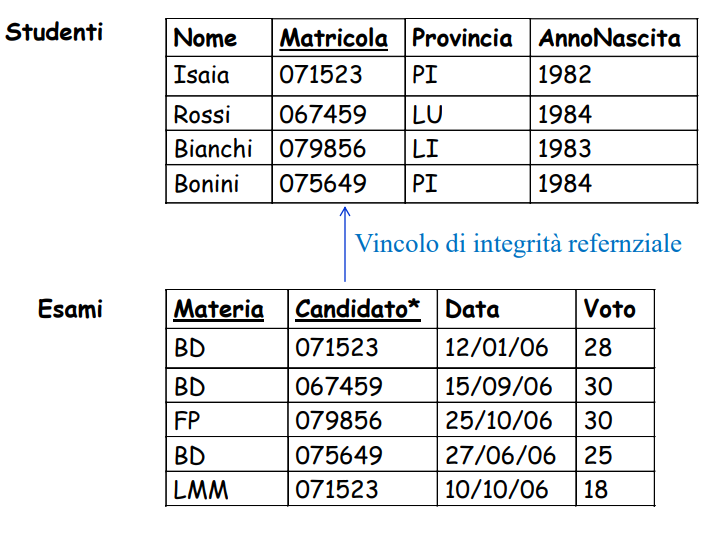
\includegraphics[scale=0.5]{integ.png}
\end{center}
\paragraph{Vantaggi}
\begin{list}{}{}
	\item \textbf{Indipendenza delle strutture fisiche} che possono cambiare dinamicamente, che potremmo avere anche con puntatori di alto livello. La rappresentazione logica dei dati (che è costituita dai soli valori) non fa riferimento a quella fisica.
	\item Si \textbf{rappresenta solo ciò che è rilevante} dal punto di vista dell'applicazione
	\item I \textbf{dati} sono \textbf{portabili} più facilmente da un sistema all'altro
	\item I \textbf{puntatori} sono \textbf{direzionali}
\end{list}
\subsection{Meccanismi}
\paragraph{Definizione} I meccanismi per definire una base di dati con il modello relazionale sono l'\textbf{ennupla} e la \textbf{relazione}.
\paragraph{Tipo ennupla} Un tipo ennupla T è un insieme finito di coppie $\langle$attributo, tipo elementare$\rangle$\\
Se T è un tipo ennupla, R(T) è lo schema della relazione R, quindi \textbf{lo schema di un DB è l'insieme di schemi di relazione R$_i$(T$_i$)}. Un'\textbf{istanza} di uno schema R(T) è un insieme finito di ennuple di tipo T.
\paragraph{Informazione incompleta} Per rappresentare un'informazione incompleta (es.: l'assenza del secondo nome) \textbf{non bisogna usare elementi del dominio} come lo 0, stringa vuota, "99"\ldots.\\
Questo perché potrebbero non esistere valori "non utilizzati", e se esistono potrebbero diventare significativi. Inoltre, in fase di utilizzo (nei programmi) bisognerebbe tenere conto ogni volta del "significato" di questi valori.\\\\
Il \textbf{valore nullo} denota l'\textbf{assenza di un valore del dominio e non è un valore del dominio}.\\
Quindi t[A] per ogni attributo A è un valore del dominio dom(A) oppure è il valore nullo NULL.\\
Si possono (e \textbf{devono}) imporre restrizioni sulla presenza di valori sulli.
\paragraph{Vincoli d'Integrità} Esistono istanze di DB che, nonostante siano sintatticamente corrette, non rappresentano informazioni possibili per l'applicazione e che quindi \textbf{generano informazioni prive di significato}. Ad esempio un voto di 32, o due studenti con la stessa matricola.\\
Uno \textbf{schema relazionale è costituito da un insieme di schemi di relazione e un insieme di vincoli d'integrità} sui possibili valori delle estensioni delle relazioni.\\
Un \textbf{vincolo d'integrità} è una \textbf{proprietà che deve essere soddisfatta dalle istanze che rappresentano informazioni corrette} per l'applicazione.
\pagebreak
\begin{list}{}{}
	\item \textbf{Vincoli Intrarelazionali}: sono vincoli che \textbf{devono essere rispettati dai valori contenuti nella relazione considerata}. Vincoli \textbf{sui valori} (o \textbf{di dominio}), vincoli \textbf{di ennupla}.
	\item \textbf{Vincoli Interrelazionali}: sono vincoli che \textbf{devono essere rispettati da valori contenuti in relazioni diverse}.
\end{list}
\paragraph{Chiave} Informalmente, una \textbf{chiave} è un \textbf{insieme di attributi che identificano le ennuple di una relazione}.\\
Formalmente, \textbf{un insieme K di attributi è \textit{superchiave} per $r$ se $r$ \textit{non} contiene due ennuple distinte $t_1$ e $t_2$ con $t_1[K] = t_2[K]$}.\\
\textbf{K è chiave per $r$ se è superchiave minimale per $r$}, cioè se non contiene altre superchiavi.\\
Un esempio classe è la matricola: è superchiave ed è un solo attributo, quindi è minimale.\\\\
Una relazione non può contenere ennuple distinte ma con valori uguali. Ogni relazione ha \textbf{sicuramente} come superchiave l'insieme di tutti gli attributi su cui è definita, quindi ogni relazione ha (almeno) una chiave.\\
L'esistenza delle chiavi garantisce l'accesso di ciascun dato della base di dati e permettono di correlare i dati in relazioni diverse.\\
Un valore nullo in una chiave non permette di identificare le ennuple o realizzare i riferimenti con altre relazioni. Una \textbf{chiave primaria} è una chiave su cui non sono ammessi valori nulli: si denota sottolineando il nome dell'attributo es. \underline{matricola}.
\paragraph{Integrità referenziale} Le informazioni in relazioni diverse sono correlate attraverso valori comuni. In particolare, \textbf{vengono prese in considerazione i valori delle chiavi primarie}, quindi le \textbf{correlazioni devono essere coerenti}.\\
Un \textbf{vincolo di integrità referenziale} (foreign key) \textbf{fra gli attributi X di una relazione R$_1$ e un'altra relazione R$_2$ impone ai valori su X in R$_1$ di comparire come valori della chiave primaria di R$_2$}.
\section{Trasformazione di schemi}
\paragraph{Progettazione logica} L'obiettivo della progettazione logica è \textbf{tradurre lo schema concettuale in uno schema logico relazionale}, che rappresenti gli stessi dati, \textbf{in maniera corretta ed efficiente}. Questo richiede una ristrutturazione del modello concettuale.
\subsection{Progettazione logica relazionale}
\paragraph{Passaggi} La progettazione di uno schema ad oggetti in uno schema relazionale avviene seguendo questi passaggi:
\begin{enumerate}
	\item rappresentazione delle associazioni 1:1 e 1:N
	\item rappresentazione delle associazioni N:M o non binarie
	\item rappresentazione delle gerarchie d'inclusione
	\item identificazione delle chiavi primarie
	\item rappresentazione degli attributi multivalore
\end{enumerate}
\paragraph{Obiettivo} Rappresentare le \textbf{stesse informazioni}, \textbf{minimizzando la ridondanza} e \textbf{producendo uno schema comprensibile} che faciliti la scrittura e la manutenzione delle applicazioni.
\subsection{Rappresentazione delle associazioni}
\paragraph{Uno a molti} Si rappresentano aggiungendo agli attributi della relazione rispetto a cui l'associazione è univoca la chiave esterna che riferisce l'altra relazione.
\begin{center}
	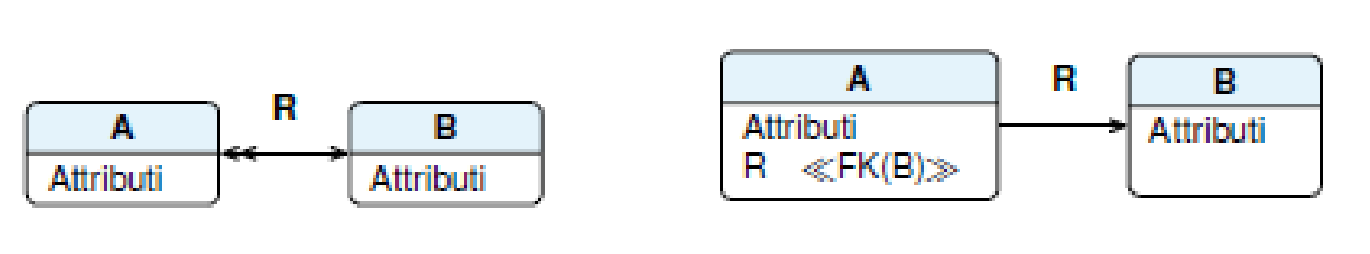
\includegraphics[scale=0.25]{ass1n.png}
\end{center}
\paragraph{Uno a uno} Si rappresentano aggiungendo la chiave esterna ad una qualunque delle due relazioni che riferisce l'altra relazione. Nel caso di un vincolo di totalità, la chiave esterna viene aggiunta alla relazione rispetto cui l'associazione è totale.
\begin{center}
	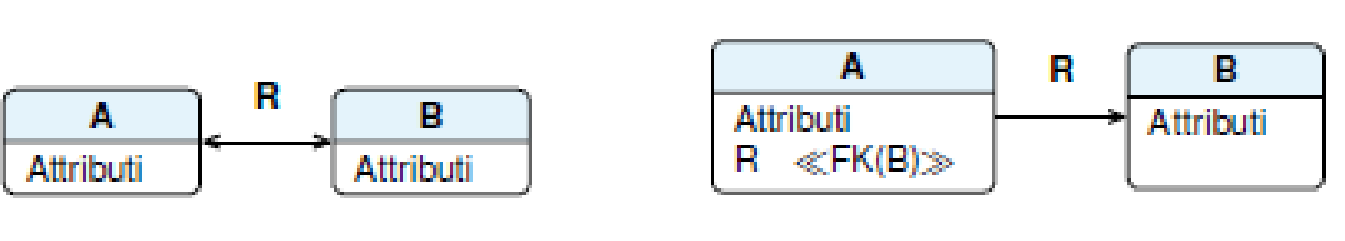
\includegraphics[scale=0.25]{ass11.png}
\end{center}
\paragraph{Molti a molti} Si rappresenta aggiungendo allo schema una nuova relazione contenente due chiavi esterne che riferiscono le due relazioni coinvolte. La chiave primaria di questa relazione è costituita dall'insieme di tutti i suoi attributi.
\begin{center}
	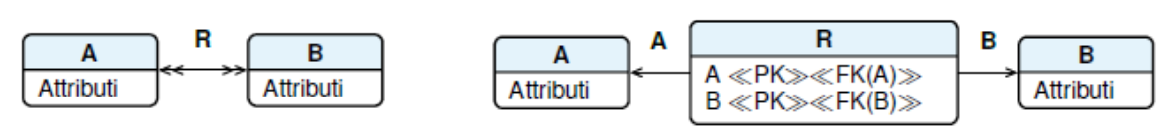
\includegraphics[scale=0.35]{assnn.png}
\end{center}
\subsection{Rappresentazione delle gerarchie fra classi}
Il modello relazionale non può rappresentare direttamente le generalizzazioni. Bisogna eliminare le gerarchie, sostituendole con classi e relazioni:
\begin{list}{}{}
	\item \textbf{Relazione unica}: accorpamento delle figlie della generalizzazione nel genitore\\
	Se $A_0$ è la classe genitore di $A_1$ e $A_2$, allora $A_1$ e $A_2$ vengono eliminate e accorpate ad $A_0$. Ad $A_0$ viene aggiunto un attributo (\textbf{discriminatore}) che indica da quale delle classi figlie deriva una certa istanza, e \textbf{gli attributi di $A_1$ e $A_2$ vengono assorbiti da $A_0$}, assumendo valore nullo sulle istanze provenienti dall'altra classe.
	\begin{center}
		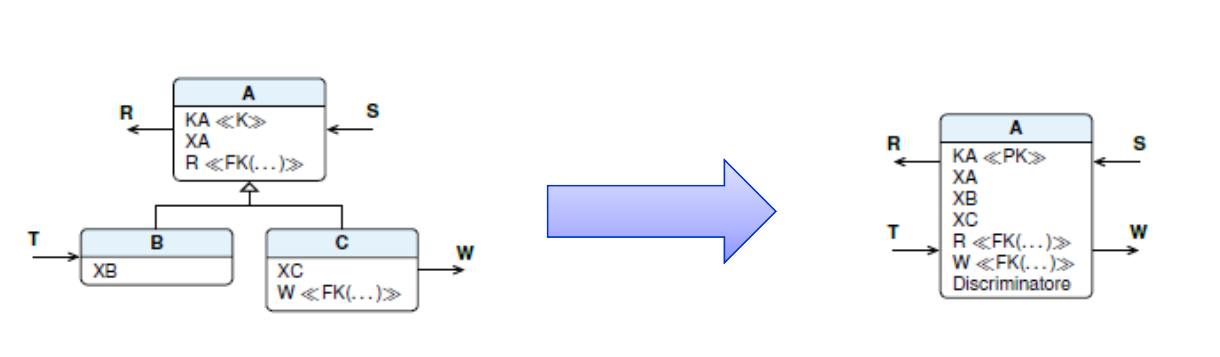
\includegraphics[scale=0.5]{relazunica.png}
	\end{center}
	\item \textbf{Partizionamento orizzontale}: accorpamento del genitore della generalizzazione nelle figlie\\
	La classe genitore $A_0$ viene eliminata e le classi figlie $A_1$ e $A_2$ ereditano le proprietà (attributi, identificatore e relazioni) della classe genitore. Le relazioni della classe genitore vengono sdoppiate, coinvolgendo ciascuna delle figlie.\\
	Divide gli elementi della superclasse in più relazioni diverse, per cui \textbf{non è possibile mantenere un vincolo referenziale verso la superclasse stessa}. Quindi, \textbf{non si usa se nello schema relazionale grafico c'è una freccia che entra nella superclasse} (come la $\leftarrow^S$ nell'esempio sopra, che entra nella superclasse $A$).
	\begin{center}
		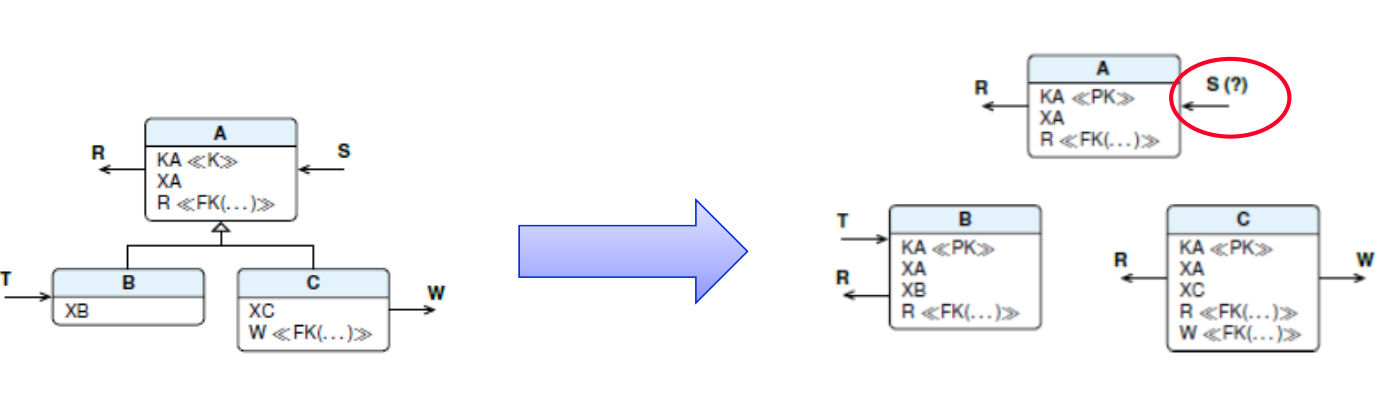
\includegraphics[scale=0.45]{partorizz.png}
	\end{center}
	\item \textbf{Partizionamento verticale}: sostituzione della generalizzazione con relazioni.\\
	La generalizzazione si trasforma in due associazioni uno ad uno che legano rispettivamente la classe progenitore con le classi figlie. In questo caso, \textbf{non c'è un trasferimento di attributi o di associazioni} e le classi figlie $A_1$ e $A_2$ sono identificate esternamente dalla classe genitore $A_0$.\\
	Nello schema ottenuto si aggiungono dei vincoli: ogni occorrenza di $A_0$ non può partecipare contemporaneamente alle due associazioni e se la generalizzazione è totale, deve partecipare almeno una delle due.
	\begin{center}
		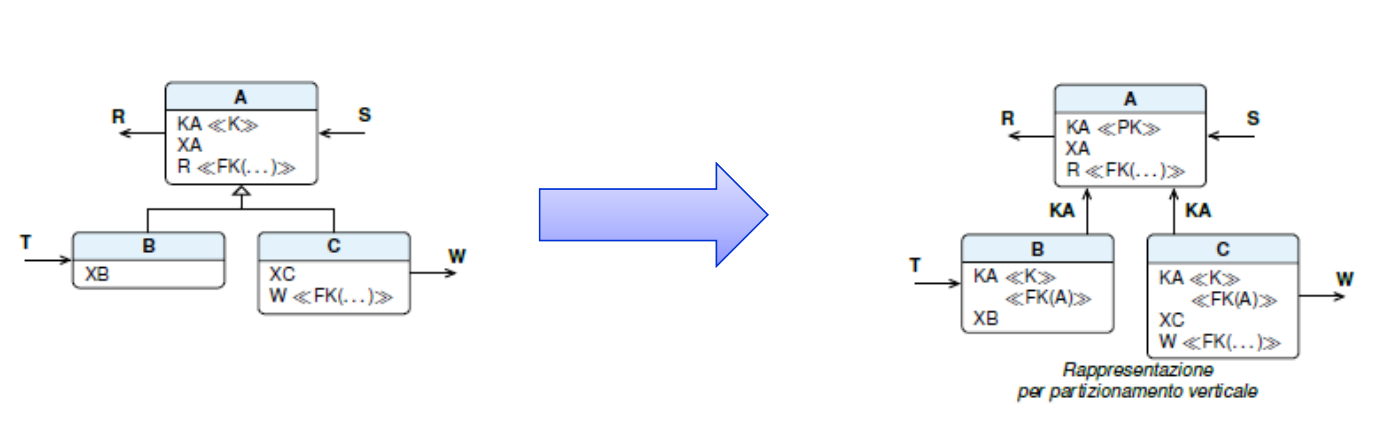
\includegraphics[scale=0.45]{partvert.png}
	\end{center}
\end{list}
\chapter{Algebra Relazionale}
\section{Linguaggi}
\paragraph{Linguaggi per i DB}
\begin{list}{}{}
	\item \textbf{DDL} \textbf{Data Definition Language}, per le \textbf{operazioni sullo schema}.\\
Operazioni di creazione, cancellazione e modifica di schemi di tabelle, creazione viste, creazione indici\ldots
	\item \textbf{DML} \textbf{Data Manipulation Language}, per le \textbf{operazioni sui dati}.\begin{list}{}{}
	\item \textbf{Data Query Language}, per le \textbf{query}, cioè l'\textbf{interrogazione del DB}
	\item \textbf{Aggiornamento dati}, per inserimento, cancellazione e modifica dei dati.
\end{list}
\end{list}
\paragraph{Linguaggi relazionali}
\begin{list}{}{}
	\item \textbf{Algebra relazionale}: insieme di operatori su relazioni che danno come risultato altre relazioni.\\
	Non si usa come linguaggio di interrogazione dei DBMS ma come rappresentazione interna delle interrogazioni.
	\item \textbf{Calcolo relazionale}: linguaggio dichiarativo di tipo logico da cui è stato derivato l'SQL.
\end{list}
\section{Operatori}
\begin{list}{}{}
	\item Unione, intersezione e differenza
	\item Ridenominazione
	\item Selezione
	\item Proiezione
	\item Join (naturale, prodotto cartesiano, theta-join)
\end{list}
Sono \textbf{operatori insiemistici}: \textbf{le relazioni sono insiemi} e i risultati devono essere relazioni a loro volta. L'unione, intersezione e differenza sono applicabili solamente a relazioni definite sugli stessi attributi, cioè \textbf{possono operare solo su tuple uniformi}.
\subsection{Ridenominazione}
\paragraph{Operatore monadico} Un solo argomento, modifica lo schema lasciando inalterata l'istanza dell'operando. Si indica con la lettera $\rho$, esempio: $\rho$ 
\textit{nomecolonna}$\leftarrow$\textit{nuovonome}
\subsection{Proiezione}
\paragraph{Operatore monadico} Produce un risultato che ha \textbf{parte degli attributi} dell'operando e \textbf{contiene ennuple cui contribuiscono tutte le ennuple dell'operando ristrette agli attributi nella lista}. Esempio $\pi_{\textsl{lista attributi}}$(\textit{operando})\\
$\pi_{A_1\ldots A_n}$(\textit{R})\\
Contiene \textbf{al più} tante ennuple quante l'operando, ma può contenerne meno. Se $X$ è superchiave di R, allora $\pi_X$(R) contiene esattamente tante ennuple quante R. Se $X$ non è superchiave, \textbf{potrebbero esistere valori ripetuti su quegli attributi}, che quindi \textbf{vengono rappresentati una sola volta}.
\pagebreak
\subsection{Selezione}
\paragraph{Operatore monadico} Produce un risultato con \textbf{lo stesso schema dell'operando}, \textbf{contiene un sottoinsieme delle ennuple dell'operando} cioè quelle che \textbf{soddisfano una condizione} espressa combinando con i connettivi logici $\wedge$, $\vee$, $\neg$, condizioni atomiche del tipo $A\Theta B$ o $A\Theta c$ dove $\Theta$ è un operatore di confronto, $A$ e $B$ sono attributi su cui l'operatore $\Theta$ abbia senso e $c$ sia una costate compatibile col dominio di $A$.\\
Viene denotata con $\sigma_{\textsl{condizione}}$(\textit{operando}), ad esempio $\sigma_{Stipendio>50\:\wedge\:Filiale='Milano'}$(Impiegati)\\
Per riferirsi ai valori nulli si usano apposite condizioni IS NULL e IS NOT NULL.\\
\begin{center}
$\sigma_{eta>30}$(Persone) $\cup\:\:\sigma_{eta\leq 30}$(Persone) $\cup\:\:\sigma_{eta\:\:IS\:NULL}$(Persone)\\
$=$\\
$\sigma_{eta>30\:\:\vee\:\:eta\leq 30\:\:\vee\:\:eta\:IS NULL}$(Persone)\\
$=$\\
Persone
\end{center}
\begin{center}
	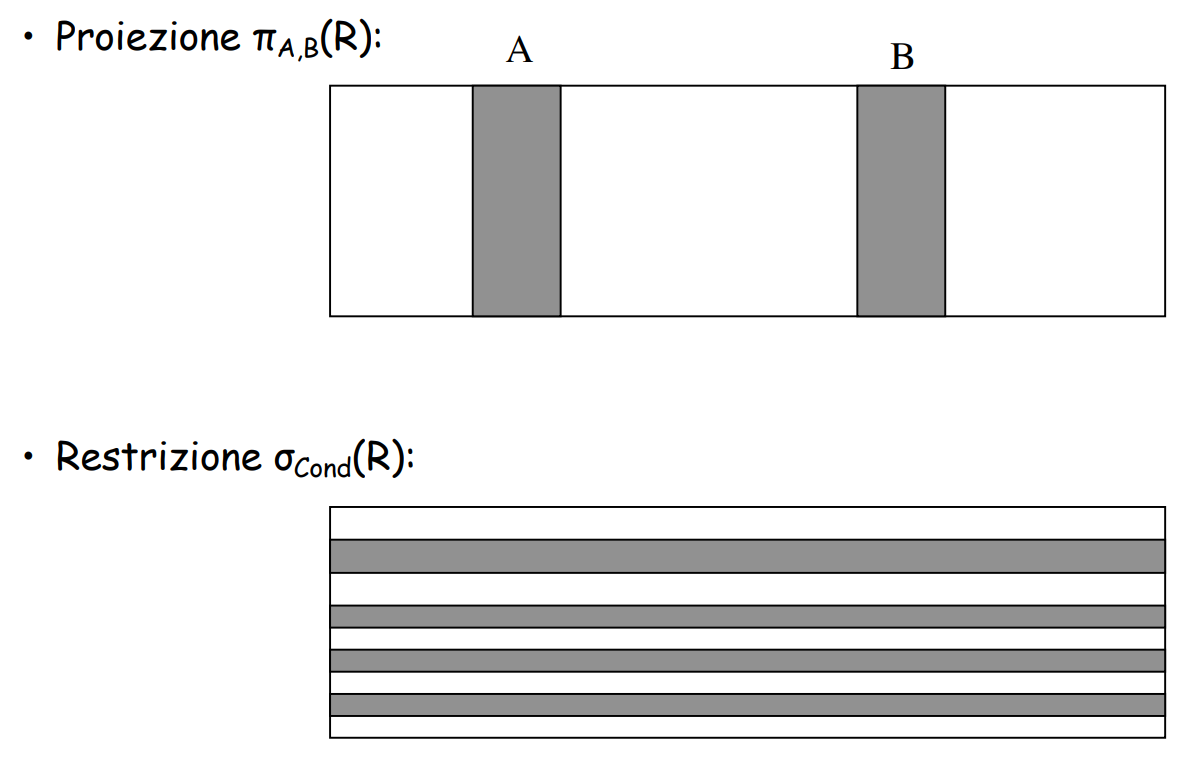
\includegraphics[scale=0.4]{proiezrestriz.png}
\end{center}
\subsection{Join}
\paragraph{Giunzione} Combinando selezione e proiezione possiamo estrarre informazioni da una relazione, ma \textbf{non possiamo correlare informazioni presenti in relazioni diverse}.\\
Il \textbf{join} è l'operatore più interessante dell'algebra relazionale perché consente di correlare i dati in relazioni diverse.
\paragraph{Join naturale} Operatore binario (generalizzabile) che \textbf{correla dati} in relazioni diverse \textbf{sulla base di valori uguali in attributi con lo stesso nome}.\\
Produce un risultato sull'unione degli attributi degli operandi con \textbf{ennuple ottenute combinando le ennuple degli operandi con valori uguali sugli attributi in comune}.\\
Dati $R_1(X_1)$, $R_2(X_2)$, allora $R_1\bowtie R_2$ è una relazione su $X_1\cup X_2$\\
$R_1\bowtie R_2 = \{t$ su $X_1\cup X_2\:|\:\exists t_1\in R_1 \wedge t_2\in R_2$ con $t[X_1] = t_1$ e $t[X_2] = t_2\}$
\subparagraph{Cardinalità} Dati $R_1(A,B)$ e $R_2(B,C)$, il join contiene un numero di ennuple compreso fra 0 e $|R_1|\cdot|R_2|$
$$0 \leq |R_1 \bowtie R_2|\leq |R_1|\cdot|R_2|$$
Se il join è completo, allora contiene un numero di ennuple almeno uguale al massimo tra $|R_1|$ e $|R_2|$. Se il join coinvolge una chiave B di $R_2$, allora $0 \leq |R_1 \bowtie R_2|\leq |R_1|$.\\
Se coinvolge una chiave B di $R_2$ e un vincolo di integrità referenziale tra attributi di $R_1$ e la chiave di $R_2$,\\allora $|R_1 \bowtie R_2| = |R_1|$
\paragraph{Join esterno} Estende con valori nulli le ennuple che verrebbero tagliate fuori da un join interno.\\
Esiste in tre versioni:
\begin{list}{}{}
	\item \textbf{Sinistro} $R \overleftarrow{\bowtie} S$, mantiene tutte le ennuple del primo operando estendendole con valori nulli se necessario.
	\item \textbf{Destro} $R \overrightarrow{\bowtie} S$, idem ma del secondo operando.
	\item \textbf{Completo}, idem ma di entrambi gli operandi.
\end{list}
\paragraph{Prodotto cartesiano} Un join naturale senza attributi in comune: contiene sempre un numero di ennuple pari al prodotto delle cardinalità degli operandi.
\paragraph{Theta-join} Il prodotto cartesiano ha senso solo se seguito da una selezione $\sigma_{condizione}(R_1\bowtie R_2)$, che viene abbreviato con $R_1\bowtie_{condizione}R_2$
\paragraph{Self-join} Non si potrebbe fare una join del tipo Genitore $\bowtie$ Genitore, perché ritornerebbe la stessa tabella Genitore poiché tutti gli attributi coincidono. Torna utile effettuare una ridenominazione del tipo $\rho_{Nonno,Genitore\leftarrow Genitore,Figlio}$(Genitore) per poi effettuare una natural join del risultato con Genitore.
\subsection{Raggruppamento} Con l'operatore $_{\{A_i\}}\gamma_{\{f_i\}}$(R) si effettura il raggruppamento.
\begin{list}{}{}
	\item $A_i$ sono gli \textbf{attributi} di R
	\item $f_i$ sono le \textbf{espressioni} che usano \textbf{funzioni di aggregazione} (min, max, count, sum\ldots)
\end{list}
Il valore del raggruppamento è calcolato come segue:
\begin{list}{}{}
	\item si partizionano le ennuple di R mettendo nello stesso gruppo tutte le ennuple con valori uguali degli $A_i$ (si \textbf{raggruppa per $A_i$})
	\item si \textbf{calcolano le espressioni $f_i$} per ogni gruppo
	\item per ogni gruppo, si \textbf{restituisce una sola ennupla con attributi i valori} degli $A_i$ e delle espressioni $f_i$
\end{list}
\begin{center}
	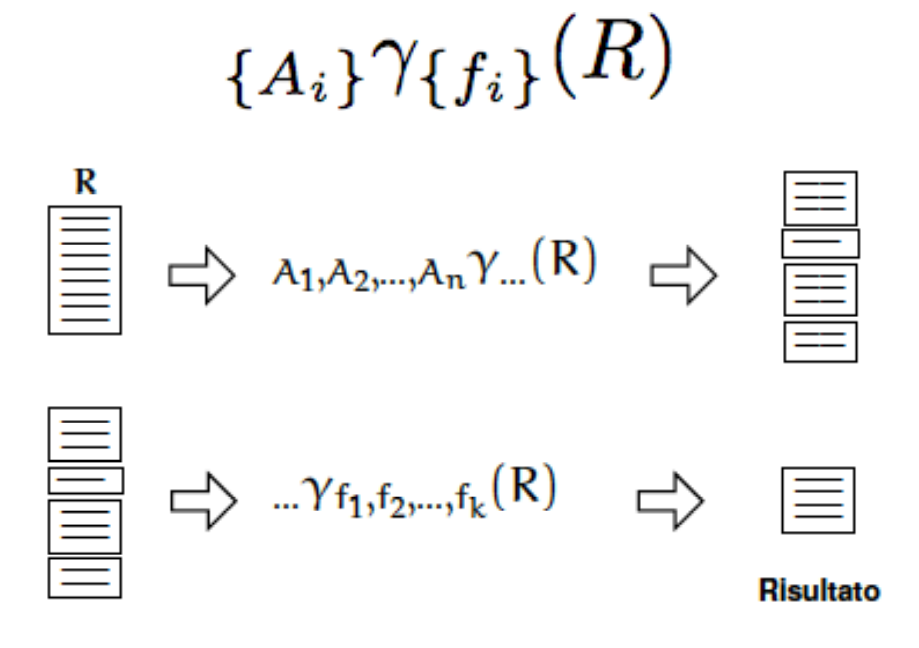
\includegraphics[scale=0.5]{raggrup.png}
\end{center}
\chapter{Interrogazione di una base di dati}
\paragraph{SQL} L'interrogazione di una base di dati è uno degli aspetti più importanti del linguaggio SQL. I comandi di interrogazione, o \textbf{query}, permettono di effettuare una ricerca dei dati presenti nel database che soddisfano particolari condizioni richieste dall'utente.
\begin{lstlisting}
SELECT	s.Nome, e.Data
FROM	Studenti s, Esami e
WHERE	e.Materia = 'BD' AND e.Voto = 30 AND e.Matricola = s.Matricola
\end{lstlisting}
\begin{lstlisting}
SELECT	s.Nome AS Nome, 2020 - s.AnnoNascita AS Eta, 0 AS NumeroEsami
FROM	Studenti s
WHERE	NOT EXISTS(SELECT * FROM Esami e WHERE e.Matricola = s.Matricola)
\end{lstlisting}
\paragraph{Storia} Definito nel 1973, SQL è oggi il linguaggio universale dei sistemi relazionali. Ci sono vari standard (SQL-84, SQL-89\ldots fino a SQL-1999 ANSI/ISO ad oggetti) ed è composto da DDL, DML e \textbf{query language}.
\paragraph{Select From Where} SQL è un \textbf{calcolo su multinsiemi}. Il comando base dell'SQL è:
\begin{lstlisting}
SELECT [DISTINCT] Attributo{, Attributo}
FROM Tabella [Ide]{, Tabella [Ide]}
[WHERE Condizione]
\end{lstlisting}
La semantica è \textbf{prodotto}, \textbf{restrizione}, \textbf{proiezione}. Un attributo A di una tabella "R x" si denota come A, R.A oppure x.A

\begin{lstlisting}
SELECT ListaAttributi
FROM ListaTabelle
[WHERE Condizione]
\end{lstlisting}
La query considera il \textbf{prodotto cartesiano tra le tabelle in \texttt{ListaTabelle}} (\textbf{join}).\\
Fra queste, \textbf{seleziona solo le righe che soddisfano la \texttt{Condizione}} (\textbf{selezione}).\\
Infine, \textbf{valuta le espressioni specificate nella target list \texttt{ListaAttributi}} (\textbf{proiezione}).\\
La SELECT quindi implementa gli operatori di proiezione, selezione e join dell'algebra relazionale.
\subsection{SELECT}
\paragraph{Proiezione} Specifica la target list, cioè corrisponde a scegliere gli attributi della/e tabella/e interessate. Implementa quindi l'operazione di \textbf{proiezione} dell'algebra relazionale.
\subsection{FROM}
\paragraph{Tabelle} Ha lo scopo di scegliere quali sono le tabelle del database da cui vogliamo estrarre le nostre informazioni. Nel caso in cui le tabelle elencate siano due, la FROM insieme alla WHERE implementa il theta-join.
\subsection{WHERE}
\paragraph{Selezione} Serve a scegliere le righe della tabella che soddisfano una certa condizione. In questo modo la clausola WHERE implementa la \textbf{selezione} dell'algebra relazionale.
\paragraph{Condizioni} In SQL sono disponibili una serie di condizioni a seconda del tipo di dato da confrontare, oltre ai IS NULL e IS NOT NULL per i dati mancanti.\\
In particolare, con l'operatore LIKE si possono effettuare ricerche con wildcard: $\%$ per zero o più caratteri, $\_$ per un carattere. Per esempio, \texttt{WHERE Nome LIKE \%a} ricercherà tutti i valori del campo \texttt{Nome} che finiscono per \texttt{a}, oppure \texttt{WHERE Sequenza LIKE \%G\_\_\_G\%} seleziona i valori dove compaiono due \texttt{G} separate da 3 caratteri.\\
Si possono inserire anche dei simboli escape, ad esempio se vogliamo cercare valori in cui compare \texttt{\%} si può scrivere \texttt{WHERE Sconto LIKE \_5\#\% ESCAPE \#}, così da trovare tutti i valori sconto con 5 nelle unità.
\section{Ordinamento e aggregazione}
\paragraph{Ordinamento} Il risultato di una SELECT si può ordinare in base ad un attributo e in maniera crescente o decrescente
\begin{lstlisting}
SELECT ListaAttributi
FROM ListaTabelle
WHERE Condizione
ORDER BY Attributo [ASC/DESC]
\end{lstlisting}
Le righe verranno ordinate in base al campo Attributo in maniera crescente (ASC) o descrescente (DESC). L'ordinamento è quello più naturale sul dominio dell'attributo (numerico, alfabetico\ldots).\\
Si possono anche fare ordinamenti multipli, ad esempio se si vuole ordinare i dati in base ad una certa chiave (attributo) e poi ordinare i dati che coincidono su quella chiave in base ad un'altra chiave (altro attributo).
\begin{lstlisting}
...
ORDER BY Attributo1 [ASC/DESC]{, Attributon [ASC/DESC]}
\end{lstlisting}
Verranno ordinati prima per Attributo1, le righe coincidenti su Attributo1 verranno ordinate per Attributo2\ldots.
\paragraph{Aggregazione} Nella target list possiamo avere anche espressioni che calcolano valori a partire da insiemi di ennuple e che restituiscono una tabella molto particolare, costituita da un \textbf{singolo valore scalare}.\\
Sono 5 gli \textbf{operatori aggregati} previsti da SQL2:
\begin{list}{}{}
	\item \texttt{COUNT()}, conteggio: restituisce il numero di righe della tabella o il numero di valori di un particolare attributo. Con \texttt{(*)} conta tutte le righe selezionate, con \texttt{ALL} conta tutti i valori non nulli delle righe selezionate, \texttt{DISTINCT} conta tutti i valori non nulli distinti delle righe selezionate. Di default è \texttt{ALL}.
	\item \texttt{MIN()}, minimo. L'argomento può essere una funziona aritmetica.
	\item \texttt{MAX()}, massimo. L'argomento può essere una funziona aritmetica.
	\item \texttt{SUM()}, somma. Le specifiche \texttt{ALL} e \texttt{DISTINCT} permettono di sommare tutti i valori non nulli o tutti i valori distinti. Anche qua di default è \texttt{ALL}.
	\item \texttt{AVG()}, media (dei valori non nulli). \texttt{ALL} e \texttt{DISTINCT} per calcolare la media fra tutti i valori o fra quelli distinti, default \texttt{ALL}.
\end{list}
Non è possibile utilizzare, in una stessa SELECT, una proiezione su alcuni attributi della tabella e operatori aggregati sulla stessa tabella. Si possono, invece, fare operazioni aggregate su colonne diverse della stessa tabella.
\paragraph{Raggruppamento} A volta può essere richiesto di calcolare operatori aggregati non per l'intera tabella ma raggruppando le righe i cui valori coincidono su un certo attributo: possiamo scrivere \texttt{GROUP BY Attributo}.\\
Con \texttt{HAVING} si possono applicare condizioni sul valore aggregato per ogni gruppo.\\
Attributo $\rightarrow$ \texttt{WHERE}\\
Operatore aggregato $\rightarrow$ \texttt{HAVING}
\section{Semantica}
La query è innanzitutto eseguita senza operatori aggregati e senza \texttt{GROUP BY}.\\
Quindi il risultato è diviso in sottoinsiemi aventi gli stessi valori per gli attributi elencati in \texttt{GROUP BY}.\\
Quindi l'operatore aggregato è calcolato su ogni sottoinsieme.
\paragraph{Osservazione} Quando si effettua un \textbf{raggruppamento}, questo \textbf{deve essere effettuato su tutti gli elementi della target list che non sono operatori aggregati} (ossia sull'insieme degli attributi puri).\\
Questo perché \textbf{nel risultato deve apparire una riga per ogni gruppo}.
\paragraph{Esempio di query} \texttt{HAVING} può essere usato solo in presenza di un \texttt{GROUP BY} e dopo di esso.
\begin{lstlisting}
SELECT		Citta, Avg(Voto)
FROM		EsamiBD
WHERE		Eta < 21
GROUP BY	Citta
HAVING		AVG(Voto) > 26
\end{lstlisting}
\begin{center}
	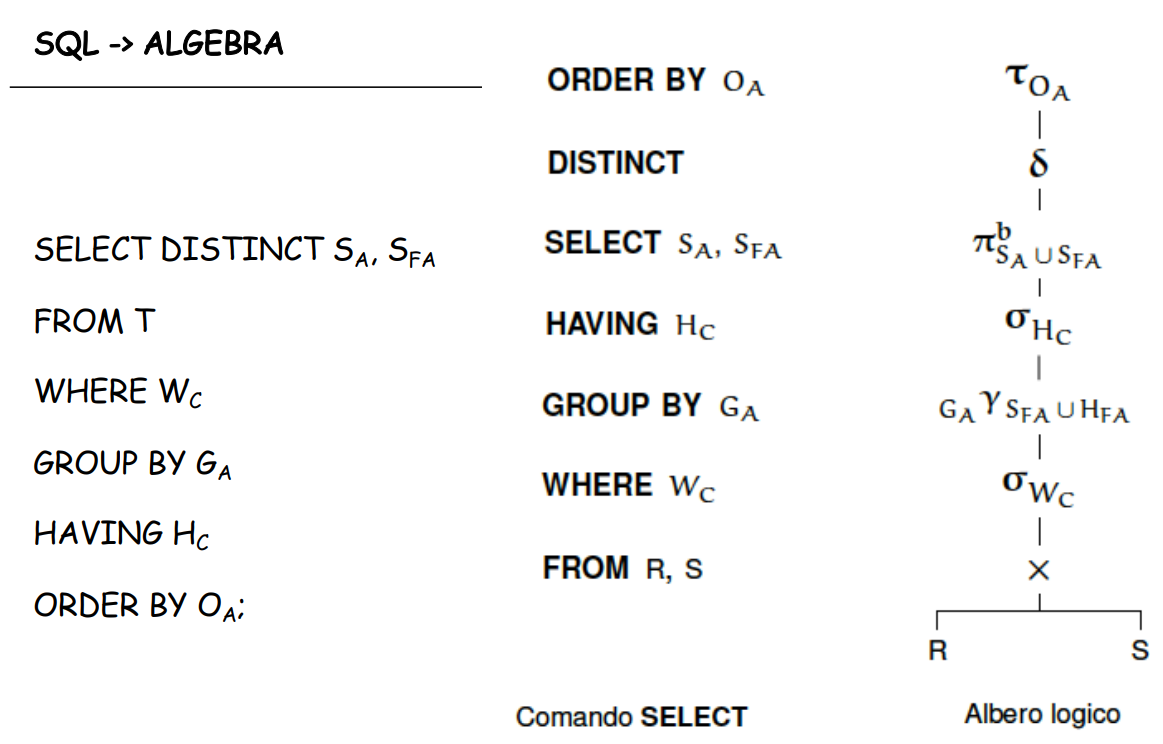
\includegraphics[scale=0.5]{sqlalg.png}
\end{center}
\section{Subquery}
Una \textbf{subquery} un comando SELECT racchiuso tra parantesi tonde ed inserito all'interno di un altro comando SQL (ad esempio un'altra query).\\
Possono essere usate nei seguenti casi:
\begin{list}{}{}
	\item in espressioni di confronto
	\item in espressioni di confronto quantificato
	\item in espressioni IN
	\item in espressioni EXISTS
	\item nel calcolo di espressioni
\end{list}
\paragraph{Tipologie} Ci sono tre tipologie di subquery:
\begin{list}{}{}
	\item \textbf{Subquery Scalare}: comando SELECT che restituisce \textbf{un solo valore}\\
	Es: \texttt{SELECT MAX(Cilindrata) FROM Veicoli}
	\item \textbf{Subquery di Colonna}: comando SELECT che restituisce \textbf{una colonna}\\
	Es: \texttt{SELECT CodCateogira FROM Veicoli}
	\item \textbf{Subquery di Tabella}: comando SELECT che restituisce \textbf{una tabella}\\
	Es: \texttt{SELECT Targa, CodMod, Posti FROM Veicoli}
\end{list}
\pagebreak
\section{Quantificazione}
Tutte le interrogazioni su di un'associazione multivalore vanno quantificate.
\begin{center}
	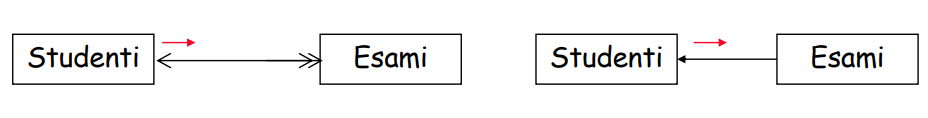
\includegraphics[scale=0.6]{quantific.png}
\end{center}
La query "gli studenti che hanno preso 30" è \textbf{ambigua}.
\begin{list}{}{}
	\item Gli studenti che hanno preso \textbf{sempre} 30: \textbf{universale}
	\item Gli studenti che hanno preso \textbf{almeno un} 30: \textbf{esistenziale}
	\item Gli studenti che \textbf{non} hanno preso \textbf{qualche} 30: \textbf{universale}
	\item Gli studenti che \textbf{non} hanno preso \textbf{sempre} 30: \textbf{esistenziale}
\end{list}
Universale negata = esistenziale\\
Esistenziale negata = universale
\paragraph{ANY, ALL, EXISTS} Le condizioni in SQL permettono il confronto fra un attributo ed il risultato di una subquery che restituisce una colonna od una tabella.
\begin{list}{}{}
	\item Operatore \textbf{scalare} (ANY $|$ ALL) \texttt{SELECT\ldots}\\
	ANY: il predicato è vero se \textbf{almeno uno dei valori restituiti dalla subquery soddisfano la condizione}
	ALL: il predicato è vero se \textbf{tutti i valori restituiti dalla subquery soddisfano la condizione}
	\item Quantificatore \textbf{esistenziale} EXISTS \texttt{SELECT\ldots}\\
	Il predicato è vero se \textbf{la subquery restituisce almeno una tupla}.
\end{list}
\section{Unione, Intersezione, Differenza}
A volte può essere utile poter ottenere un'unica tabella contenente alcuni dei dati contenuti in due tabelle omogenee, ossia con attributi definiti sullo stesso dominio.\\
La SELECT da sola non permette di fare questo tipo di operazioni su tabelle. Esistono per questo dei costrutti espliciti che utilizzano le parole chiave UNION, INTERSECT, EXCEPT (o MINUS).\\
Tali operatori lavorano sulle tabelle come se fossero insiemi di righe, dunque i duplicati vengono eliminati anche dalle proiezioni (a meno di non specificare ALL).\\
Questi operatori vanno in mezzo a due SELECT:
\begin{lstlisting}
SELECT...
(UNION | INTERSECT | EXCEPT) [ALL]
SELECT...
\end{lstlisting}
\paragraph{UNION} Realizza l'operazione di unione definita nell'algebra relazionale. Utilizza come operandi le due tabelle risultanti da comandi SELECT e restituisce una terza tabella che contiene \textbf{tutte le righe della prima e della seconda tabella}.\\
Nel caso in cui dall'unione e dalla proiezione risultassero delle righe duplicate, UNION ne mantiene una sola copia (a meno di aver specificato ALL dopo UNION).\\
\textbf{Mantiene i nomi delle colonne del primo operando}. Quindi, se si vuole ridenominare, è bene ridenominare tutte le colonne che vogliamo.
\paragraph{INTERSECT} Utilizza come operandi due tabelle risultati dai comandi SELECT e restituisce una tabella che contiene \textbf{le righe comuni alle due tabelle iniziali}. Anche qua con ALL mantiene i duplicati, e realizza l'interrsezione dell'algebra relazionale.
\paragraph{EXCEPT} Utilizza come operandi due tabelle ottenute mediante due SELECT, ed ha come risultato una nuova tabella che contiene \textbf{tutte le righe della prima che non si trovano nella seconda}. Realizza la differenza dell'algebra relazionale, ed anche qua si possono mantenere i duplicati utilizzando ALL.
\chapter{Modifica di una base di dati}
\section{Modifica dei dati}
\paragraph{Data Manipulation Language} Introduciamo ora il DML, ossia il linguaggio SQL che serve per \textbf{inserire, modificare e cancellare i dati} del database ma anche per \textbf{interrogare il database} per estrarne i dati.\\
Inizieremo descrivendo le istruzioni che servono a inserire, cancellare e modificare i dati, per poi introdurre le istruzioni per estrarre dal database le informazioni che ci interessano.
\paragraph{INSERT} Per inserire un nuovo dato in una tabella si usa INSERT INTO\ldots VALUES
\begin{lstlisting}
INSERT INTO Tabella [(ListaAttributi)] (VALUES (ListaValori) | Subquery)
\end{lstlisting}
\paragraph{Update} Si possono aggiornare alcuni dati con UPDATE
\begin{lstlisting}
UPDATE Tabella SET Attributo = Expr{, Attributo = Expr} WHERE Condizione
\end{lstlisting}
\paragraph{DELETE} Per cancellare righe dalle tabelle si usa la DELETE
\begin{lstlisting}
DELETE FROM Tabella [WHERE Condizione]
\end{lstlisting}
Per eliminare un elemento bisogna individuare quale, stabilito con la clausola WHERE con la condizione che individua l'elemento (o gli elementi) da eliminare.\\
Un particolare elemento può essere individuato dal suo valore nella chiave primaria.
\section{Definizione degli oggetti}
\paragraph{Data Definition Language} Introduciamo il DDL, cioè il linguaggio SQL che consiste nell'\textbf{insieme delle istruzioni che permettono la creazione, modifica e cancellazione delle tabelle, dei domini e degli altri oggetti del database} al fine di \textbf{definire il suo schema logico}.
\paragraph{Definizione delle tabelle} Le tabelle vengono definite in SQL con l'istruzione \textbf{CREATE TABLE}. Questa istruzione \textbf{definisce uno schema di relazione}, ne \textbf{specifica attributi, domini e vincoli} e ne crea un'istanza vuota.
\begin{lstlisting}
CREATE TABLE NomeTabella
	(NomeColonna1 TipoColonna1 ClausolaDefault1 VincoloColonna1,
	 NomeColonna2 TipoColonna2 ClausolaDefault2 VincoloColonna2,
	 ...
	 NomeColonnak TipoColonnak ClausolaDefaultk VincoloColonnak,
	 VincoliDiTabella
	)
\end{lstlisting}
CREATE TABLE è seguito dal nome della tabella e dalla \textbf{lista delle colonne} (attributi), di cui vengono specificate le caratteristiche. Alla fine si possono anche specificare eventuali vincoli di tabella, di cui parleremo.\\
La CREATE TABLE definisce uno schema di relazione e ne crea un'istanza vuota specificando attributi, domini e vincoli. Una volta create, la tabella è \textbf{pronta} per l'inserimento dei dati (che dovranno soddisfare i vincoli imposti).\\
Lo schema di una tabella, dopo che è stata creata, può essere visualizzato con \textbf{DESCRIBE NomeTabella}.
\pagebreak
\paragraph{Un linguaggio per tanti usi} SQL non è solo un query language, ma anche un linguaggio
\begin{list}{}{}
	\item per la definizione di DB (DDL)
	\begin{lstlisting}
	CREATE SCHEMA Nome AUTHORIZATION Utente
	CREATE TABLE
	CREATE INDEX
	CREATE PROCEDURE
	CREATE TRIGGER
	\end{lstlisting}
	\item per stabilire controlli sull'uso dei dati
	\begin{lstlisting}
	GRANT
	\end{lstlisting}
	\item per la modifica dei dati
\end{list}
\subsection{Tipi}
\paragraph{Tipi} I tipi più comuni per i valori sono:
\begin{list}{}{}
	\item \textbf{CHAR(n)} per stringhe di caratteri di lunghezza fissa $n$
	\item \textbf{VARCHAR(n)} per stringhe di caratteri di lunghezza variabile fino ad un massimo di $n$
	\item \textbf{INTEGER} per interi con la dimensione uguale alla parola di memoria standard dell'elaboratore
	\item \textbf{REAL} per numeri reali con dimensione uguale alla parola di memoria standard dell'elaboratore
	\item \textbf{NUMBER(p,s)} per numeri con $p$ cifre di cui $s$ decimali
	\item \textbf{FLOAT(p)} per numeri binari in virgola mobile con almeno $p$ cifre significative
	\item \textbf{DATE} per valori che rappresentano istanti nel tempo (in alcuni sistemi come Oracle) oppure solo date (con un altro tipo \textbf{TIME} per indicare l'orario)
\end{list}
\paragraph{Un esempio} 
\begin{lstlisting}
CREATE TABLE Impiegati
	(Codice CHAR(8) NOT NULL,
	 Nome CHAR(20),
	 AnnoNascita INTEGER CHECK (AnnoNascita < 2000),
	 Qualifica CHAR(20) DEFAULT 'Impiegato',
	 Supervisore CHAR(8),
	 PRIMARY KEY pk_impiegato (Codice),
	 FOREIGN KEY fk_Impiegati (Supervisore) REFERENCES Impiegati
	)
	
CREATE TABLE FamiliariACarico
	(Nome CHAR(20),
	 AnnoNascita INTEGER,
	 GradoParentela CHAR(10),
	 CapoFamiglia CHAR(8)
	 FOREIGN KEY fk_FamiliariACarico (CapoFamiglia) REFERENCES Impiegati
	)
\end{lstlisting}
\paragraph{Eliminare e modificare} Ciò che viene creato con ALTER TABLE può essere eliminato con \textbf{DROP} o modificato con \textbf{ALTER}. Con \textbf{ALTER TABLE} nello standard SQL è possibile
\begin{list}{}{}
	\item Aggiungere una colonna \textbf{ADD COLUMN}
	\item Rimuovere una colonna \textbf{DROP COLUMN}
	\item Modificare una colonna \textbf{MODIFY}
	\item Aggiungere l'assegnazione di valori di default \textbf{SET DEFAULT} o eliminarli \textbf{DROP DEFAULT}
	\item Aggiungere vincoli di tabella \textbf{ADD CONSTRAINT} o eliminarli \textbf{DROP CONSTRAINT}
	\item Altre opzioni specifica dei linguaggi.
\end{list}
\chapter{Viste}
\paragraph{Viste logiche} Le \textbf{view} possono essere definite come delle \textbf{tabelle virtuali}: i dati sono riaggregazioni dei dati contenuti nelle tabelle "fisiche" (unici veri contenitori dei dati). Le viste \textbf{non contengono fisicamente i dati ma forniscono una visione diversa, dinamicamente aggiornata, degli stessi dati delle tabelle fisiche}.\\\\
\textbf{Appare all'utente come una normale tabella}, in cui può effettuare interrogazioni e modifiche all'interno dei suoi privilegi.
\paragraph{Vantaggi} 
\begin{list}{}{}
	\item \textbf{Semplificano la rappresentazione dei dati}.\\
	Oltre ad assegnare un nome ad una vista, la sintassi dell'istruzione \textbf{CREATE VIEW} consente di cambiare i nomi delle colonne.\\
	In generale, uno dei requisiti per la progettazione di un DB è la \textbf{normalizzazione dei dati}. La forma normalizzata di un DB, sebbene permetta una corretta modellazione della realtà, a volte porta ad una \textbf{maggiore difficoltà di comprensione dei dati da parte dell'utente}. Le viste consentono quindi di fornire i dati all'utente in una forma più intuitiva. Consentono anche di \textbf{convertire le unità di misura e creare nuovi formati}.
	\item Possono essere \textbf{convenienti per eseguire query molto complesse}.
	\item Consentono di \textbf{proteggere il database}: le viste ad accesso limitato possono essere usate per \textbf{controllare le informazioni a cui accede un determinato utente} del database.
	\item \textbf{Indipendenza logica}\\
	Consentono di operare modifiche allo schema del database senza modificare le applicazioni che lo utilizzano se passano attraverso le viste. Un po' come le interfacce nell'OOP.
\end{list}
\paragraph{Limitazioni}
\begin{list}{}{}
	\item Non consentono l'utilizzo degli operatori booleani UNION, INTERSECT ed EXCEPT.\\
	Gli ultimi due possono essere realizzati mediante una semplice SELECT, ma lo stesso non si può dire di UNION.
	\item Non è possibile usare ORDER BY.
\end{list}
\paragraph{Sintassi} Il comando DDL che consente di definire una vista è 
\begin{lstlisting}
CREATE VIEW NomeVista [(ListaAttributi)] AS Subquery [WITH [LOCAL | CASCADED] CHECK OPTION]
\end{lstlisting}
I nomi delle colonne nella ListaAttributi sono assegnati alle colonen della vista, che corrispondono \textbf{ordinatamente} alle colonne elencate nella SELECT della subquery.\\
Se questi non sono specificati, le colonne della vista assumono gli stessi nomi di quelli della/e tabella/e a cui si riferisce.\\
Di seguito un esempio
\begin{lstlisting}
CREATE VIEW ImpiegatiAmmin (Matricola, Nome, Cognome, Stipendio)
AS	(SELECT Matri, Nome, Cognome, Stip
	 FROM Impiegato
	 WHERE Dipart = 'Amministrazione' AND Stipendio > 1000
	)
\end{lstlisting}
Nonostante il \textbf{contenuto} sia \textbf{dinamico}, la \textbf{struttura non lo è}. Se una vista è definita su una subquery che riferisce una tabella T a cui viene aggiunta una colonna, la definizione \textit{non} viene estesa alla vista. Ossia la vista conterrà sempre le stesse colonne che aveva prima dell'inserimento della nuova colonna in T.
\paragraph{Vista di gruppo} Una \textbf{vista di gruppo} è una vista in cui una delle colonne è una funzione di gruppo. Diventa obbligatorio assegnare un nome alla colonna della vista corrispondente alla funzione di gruppo. Un esempio:
\begin{lstlisting}
CREATE VIEW A3 (CodFabbrica, NumVersioni)
AS	(SELECT CodFabbrica, SUM(NumVersioni)
	 FROM Modelli
	 GROUP BY CodBFabbrica
	)
\end{lstlisting}
È una vista di gruppo anche una vista definita in base ad una vista di gruppo
\begin{lstlisting}
CREATE VIEW A4
AS	(SELECT NumVersioni
	 FROM A3
	)
\end{lstlisting}
\paragraph{Eliminare le viste} Le viste si eliminano con il comando
\begin{lstlisting}
DROP NomeViste [RESTRICT | CASCADE]
\end{lstlisting}
\begin{list}{}{}
	\item \textbf{RESTRICT}: la vista viene eliminata solo se non è riferita nella definizione di altri oggetti.
	\item \textbf{CASCADE}: la vista viene eliminata e vengono eliminate tutte le dipendenze da tale vista nelle altre definizioni dello schema.
\end{list}
Nell'esempio, \textbf{DROP VIEW A3 CASCADE} elimina anche A4 oltre ad A3, mentre\\\textbf{DROP VIEW A3 RESTRICT} impedisce la cancellazione di A3 finché A4 è presente nello schema.
\paragraph{Viste modificabili} Le viste si interrogano come le tabelle, ma \textbf{in generale non sono modificabili}. Per poterlo fare, \textbf{deve esistere una corrispondenza biunivoca fra le righe della vista e le righe di una tabella} di base ovvero:
\begin{list}{}{}
	\item SELECT senza DISTINCT e solo di sttributi
	\item FROM una sola tabella modificabile
	\item WHERE senza sottoquery
	\item GROUP BY e HAVING non presenti nella definizione
\end{list}
Si potrebbe aggiornare direttamente le tabelle collegate, ma \textbf{ha senso aggiornare le view nel case di accesso dati controllato}.
\paragraph{CHECK OPTION} L'opzione WITH CHECK OPTION messa alla fine della definizione della vista assicura che le operazioni di inserimento e modifica effettuate tramite la vista soddisfino la clausola WHERE della subquery.\\\\
Supponiamo che una vista V1 sia definita in termini di un'altra vista V2. Se V1 è creata con WITH CHECK OPTION, il \textbf{DBMS verifica che la nuova tupla t inserita soddisfi sia la definizione di V1 che quella di V2} (e di tutte le altre eventuali viste da cui V1 dipende), \textbf{indipendentemente dal fatto che V2 sia definita con} WITH CHECK OPTION.\\
Questo comportamento di default è equivalente a WITH \textbf{CASCADED} CHECK OPTION. Lo si può alterare definendo V1 WITH \textbf{LOCAL} CHECK OPTION, così facendo il DBMS verifica solo che t soddisfi la specifica di V1 e di tutte e sole le viste da cui V1 dipende per cui è stata specificata WITH CHECK OPTION.
\chapter{Vincoli}
\section{Vincoli Intrarelazionali}
\paragraph{Integrità} I \textbf{vincoli di integrità} consentono di \textbf{limitare i valori ammissibili per una determinata colonna della tabella in base a specifici criteri}.\\
I \textbf{vincoli di integrità intrarelazionali}, ossia che non fanno riferimento ad altre relazioni, sono:
\begin{list}{}{}
	\item NOT NULL
	\item UNIQUE, definisce chiavi\\
	Può essere espresso in due forme:
	\begin{list}{}{}
		\item Nella definizione di un attributo, se forma da solo la chiave.\\
		Usato nella definizione dell'attributo, UNIQUE indica che non ci possono essere due valori uguali in quella colonna: è una chiave della relazione, ma non una chiave primaria.
		\item Come elemento separato.\\
		Può essere riferito anche a insiemi di attributi: ciò significa che non ci devono essere due righe per cui l'insieme dei valori corrispondenti agli attributi specificati siano uguali. In questo caso è dichiarato dopo la specifica delle colonne con UNIQUE (ListaAttributi)
	\end{list}
	\item PRIMARY KEY, chiave primaria. Una sola e implica il NOT NULL e l'UNIQUE.\\
	Questo vincolo è simile a UNIQUE, ma definisce la chiave primaria della relazione ossia \textbf{un attributo che individua univocamente il dato}. Anche qua abbiamo due forme:
	\begin{list}{}{}
		\item Nella definizione di un attributo, se forma da solo la chiave.		
		\item Come elemento separato, nel caso di chiave primaria formata da più attributi.
	\end{list}
	\item CHECK, vedremo più avanti
\end{list}
\section{Vincoli Interrelazionali}
\paragraph{Referenziali} Sono quei vincoli che vengono imposti quando \textbf{gli attributi di due diverse tabelle devono essere messi in relazione}. Questo viene fatto per soddisfare l'esigenza di DB \textbf{non ridondanti} e per \textbf{mantenere i dati sincronizzati}.\\
Se due tabelle gestiscono gli stessi dati, \textbf{è bene che di essi non ce ne siano più copie} sia per non occupare troppa memoria sia per non modificare due volte lo stesso dato per mantenere la coerenza.\\\\
REFERENCES e FOREIGN KEY permettono di definire i \textbf{vincoli di integrità referenziale}. Anche qua due sintassi:
\begin{list}{}{}
	\item Per singoli attributi, come vincolo di colonna
	\begin{lstlisting}
Attributok REFERENCES TabellaEsterna(ColonnaRiferita)
	\end{lstlisting}
	\item Per insiemi di attributi, come vincolo di tabella
	\begin{lstlisting}
FOREIGN KEY (ColonneInterne) REFERENCES TabellaEsterna(ColonneRiferite)
	\end{lstlisting}
\end{list}
\subsection{Reazione alla violazione}
Possiamo definire \textbf{politiche di reazione alla violazione}, ossia stabilire l'azione che il DBMS esegue quando si viola il vincolo. Questo può succedere quando si cancella o modifica una riga.\\
Tali reazioni vengono dichiarate al momento della definizione dei vincoli di foreign key rispettivamente mediante ON DELETE e ON UPDATE
\begin{lstlisting}
Attributok REFERENCES TabellaEsterna(ColonnaRiferita)
	[ON DELETE | ON UPDATE Reazione]

FOREIGN KEY (ColonneInterne) REFERENCES TabellaEsterna(ColonneRiferite)
	[ON DELETE | ON UPDATE Reazione]
\end{lstlisting}
\paragraph{Reazioni alla DELETE}\begin{list}{}{}
	\item NO ACTION: impedisce il delete (default)
	\item CASCADE: genera un delete a catena su tutte le righe dipendenti
	\item SET NULL: assegna NULL ai valori della colonna che ha il vincolo referenziale
	\item SET DEFAULT: assegna il valore di default ai valori della colonna che ha il vincolo referenziale
\end{list}
\paragraph{Reazioni alla UPDATE}\begin{list}{}{}
	\item NO ACTION: impedisce gli aggiornamenti che violano l'integrità referenziale (default)
	\item CASCADE: i referenti vengono impostati al nuovo valore del riferito
	\item SET NULL: i referenti vengono impostati a NULL
	\item SET DEFAULT: i referenti vengono impostati al valore di default
\end{list}
\section{CHECK}
Un vincolo di \textbf{CHECK} richiede che una colonna o un insieme di colonne \textbf{soddisfi una condizione per ogni riga della tabella}. Il vincolo specificato deve essere un'espressione booleana che è valutata usando i valori della colonna che vengono inseriti o aggiornati nella riga.\\
Può essere espresso come vincolo di colonna se coinvolge un solo attributo, oppure come vincolo di tabella se coinvolge più attributi.
\chapter{Trigger}
Un \textbf{trigger} definisce un'\textbf{azione che il database deve attivare automaticamente quando si verifica un determinato evento nel database}. Possono essere usati per \textbf{migliorare l'integrità referenziale dichiarativa}, \textbf{imporre regole complesse} oppure \textbf{effettuare revisioni sulle modifiche} dei dati.
\paragraph{DML ma anche DDL} L'\textbf{esecuzione è trasparente} all'utente e \textbf{vengono eseguiti automaticamente} quando specifici tipi di comandi (\textbf{eventi}) di manipolazione dei dati vengono eseguiti su specifiche tabelle.\\
Tali comandi comprendono i comandi DML INSERT, UPDATE e DELETE, ma gli ultimi DBMS prevedono trigger anche su alcune istruzioni DDL.\\
Anche gli aggiornamenti di specifiche colonne possono essere usati come trigger di eventi.
\section{Struttura}
I trigger si basano sul paradigma \textbf{Evento-Condizione-Azione} (\textbf{ECA})
\begin{lstlisting}
CREATE TRIGGER NomeTrigger
TipoDiTrigger Evento {, Evento}
ON TabellaTarget
[FOR EACH ROW]
[WHEN Condizione]
Azione
\end{lstlisting}
\begin{list}{}{}
	\item TipoDiTrigger: BEFORE o AFTER
	\item Evento: INSERT/DELETE/UPDATE
	\item Se si vuole specificare il trigger a livello di riga si mette anche FOR EACH ROW, altrimenti niente
	\item Condizione che si deve verificare affinché il trigger venga eseguito
	\item Azione, definita dal codice da eseguire se si verifica la condizione
\end{list}
Un esempio:
\begin{lstlisting}
CREATE TRIGGER ControlloStipendio BEFORE INSERT ON Impiegati
DECLARE StipendioMedio FLOAT
BEGIN
	SELECT AVG(Stipendio) INTO StipendioMedio
	FROM Impiegati
	WHERE Dipartimento = :new.Dipartimento;
	IF :new.Stipendio > 2 * StipendioMedio THEN
		RAISE_APPL_ERR('Stipendio Alto')
	END IF;
END;
\end{lstlisting}
\section{Tipi di trigger}
\subsection{Trigger a livello di riga}
Vengono eseguiti \textbf{una volta per ogni riga modificata in una transazione}. Spesso usati in applicazioni di revisione dei dati e si rivelano utili per \textbf{operazioni di audit dei dati} e per \textbf{mantenere sincronizzati i dati distribuiti}.\\
Si creano con la clausola \textbf{FOR EACH ROW} nel CREATE TRIGGER.
\subsection{Trigger a livello di istruzione}
Vengono eseguiti \textbf{una volta per ciascuna transazione}, indipendentemente dal numero di righe che vengono modificate.\\
Vengono usati per \textbf{attività correlate ai dati} come per \textbf{imporre misure aggiuntive di sicurezza sui tipi di transazione che possono essere eseguiti su una tabella}.\\
Questo è il \textbf{tipo di trigger predefinito} del CREATE TRIGGER, non serve specificare clausole.

\paragraph{BEFORE/AFTER} I trigger possono essere eseguiti prima o dopo l'utilizzo dei comandi, e all'interno e possibile riferire i vecchi e nuovi valori coinvolti nella transazione.\\
In caso di BEFORE, i valori \textbf{vecchi sono i valori attualmente nella tabella da modificare} e i \textbf{nuovi sono quelli che vogliamo inserire}.\\
In caso di AFTER, i valori \textbf{vecchi sono quelli che c'erano prima della modifica} mentre i \textbf{nuovi sono quelli presenti nella tabella alla fine della modifica}.
\paragraph{Attivi/Passivi} Un trigger è \textbf{attivo quando modifica lo stato della base dei dati}, mentre è \textbf{passivo quando serve a provocare il fallimento della transazione sotto certe condizioni}.
\chapter{Controllo degli accessi}
Ogni componente dello schema può essere protetto: tabelle, attributi, viste, domini\ldots\\
Il possessore della risorsa assegna dei privilegi agli altri utenti. Un utente predefinito (\_system) rappresenta l'amministratore della base di dati ed ha completo accesso alle risorsa. Ogni privilegio è caratterizzato da:
\begin{list}{}{}
	\item la risorsa a cui si riferisce
	\item l'utente che concede il privilegio
	\item l'utente che riceve il privilegio
	\item l'azione che viene permessa sulla risorsa
	\item se il privilegio può essere trasmesso o meno ad altri utenti
\end{list}
\paragraph{Tipi di privilegi}
\begin{list}{}{}
	\item SELECT: lettura dei dati
	\item INSERT: inserire record
	\item DELETE: cancellazione record
	\item UPDATE: modifica record
	\item REFERENCES: definire chiavi esterne
	\item WITH GRANT OPTION: si possono trasferire i privilegi ad altri utenti
\end{list}
I privilegi si \textbf{garantiscono} con
\begin{lstlisting}
GRANT (Privilegi | ALL PRIVILEDGES) ON Oggetto TO Utenti [WITH GRANT OPTION]
\end{lstlisting}
e si possono \textbf{revocare} (solo chi li ha garantiti) con
\begin{lstlisting}
REVOKE [GRANT OPTION FOR] Privilegi ON Oggetto FROM Utenti [CASCADE]
\end{lstlisting}
La revoca di default è RESTRICT (non esegue il comando se la revoca dei privilegi all'utente comporti qualche altra revoca), CASCADE invece forza l'esecuzione. Quando si toglie un privilegio a U, lo si toglie anche a tutti coloro che lo hanno avuto solo da U (\textit{attenzione agli effetti a catena})
\chapter{Programmazione}
\section{Uso di SQL da programmi}
\subsection{Problemi} Le problematiche principali che si incontrano quando si programmano applicazioni che comunicano con DB sono:
\begin{list}{}{}
	\item come \textbf{collegarsi al DB}
	\item come \textbf{trattare gli operatori} SQL
	\item come \textbf{trattare il risultato di un comando} SQL, cioè \textbf{le relazioni}
	\item come \textbf{scambiare informazioni sull'esito delle operazioni}
\end{list}
\subsection{Approcci}
\paragraph{Linguaggio integrato (dati e DML)} Linguaggio \textbf{disegnato ad-hoc per usare SQL}. I \textbf{comandi} SQL sono \textbf{controllati staticamente} dal traduttore ed \textbf{eseguiti dal DBMS}. Un esempio:
\subsubsection{PL/SQL, Oracle}
\paragraph{Un linguaggio integrato} Un linguaggio per manipolare DB che integra DML (SQL) con il linguaggio ospite. \textbf{Linguaggio a blocchi} con una struttura del controllo completa che \textbf{contiene l'SQL come sottolinguaggio}.\\
Permette di:
\begin{list}{}{}
	\item definire variabili di tipo scalare, record (annidato), insieme di scalari, insieme di record piatti, cursore
	\item definire i tipi delle variabili a partire da quelli del DB
	\item eseguire interrogazioni SQL ed esplorarne il risultato
	\item modificare un DB
	\item definire procedure e moduli
	\item gestire il flusso del controllo, le transazioni, le eccezioni
\end{list}
\paragraph{Linguaggio convenzionale + API} Linguaggio convenzionale che \textbf{usa delle funzioni di libreria per usare SQL}. I \textbf{comandi} SQL sono \textbf{stringhe passate come parametri alle funzioni}, che poi vengono \textbf{controllate dinamicamente} dal DBMS prima di eseguirle.\\
Quindi invece di modificare il compilatore di un linguaggio, si usa una libreria di funzioni/oggetti che operano su DB (API), alle quali si passa come parametro stringhe SQL e ritornano il risultato sul quale si opera con una logica ad iteratori. Qualche esempio:
\begin{list}{}{}
	\item \textbf{Microsoft ODBC}, C/C++ standard per Windows
	\item \textbf{Sun JDBC}, l'equivalente Java
\end{list}
Dovrebbero essere \textbf{indipendenti dal DBMS}: un \textbf{driver} gestisce le richieste e le traduce in codice specifico per il singolo DBMS. Il DB può essere in rete.
\paragraph{Linguaggio che ospita l'SQL} Linguaggio convenzionale \textbf{esteso con un nuovo costrutto per marcare i comandi} SQL. Occorre un \textbf{pre-compilatore} che \textbf{controlla i comandi SQL}, li \textbf{sostituisce con chiamate a funzioni predefinite} e \textbf{genera un programma in linguaggio convenzionale + API}.
\paragraph{Cursore} Meccanismo per ottenere uno alla volta gli elementi di una relazione. Un cursore viene definito con un'espressione SQL poi:
\begin{list}{}{}
	\item si apre per far calcolare al DBMS il risultato, poi
	\item con un opportuno comando si trasferiscono i campi delle ennuple in opportune variabili del programma
\end{list}
\begin{center}
	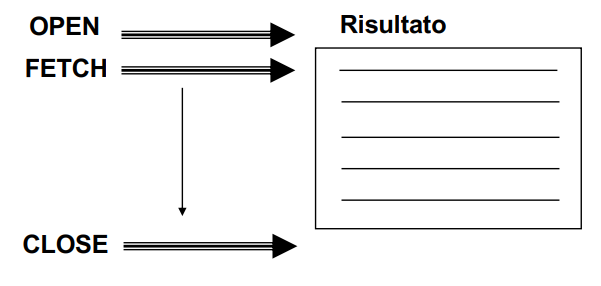
\includegraphics[scale=0.5]{cursore.png}
\end{center}
\chapter{Normalizzazione}
\section{Teoria relazionale}
\paragraph{Introduzione} Ci sono due metodi per produrre uno schema relazionale:
\begin{list}{}{}
	\item Partire da un buon schema ad oggetti e tradurlo
	\item Partire da uno schema relazionale già esistente e modificarlo o completarlo
\end{list}
\textbf{Teoria della progettazione relazionale}: si studia cosa sono le "\textbf{anomalie}" e \textbf{come eliminarle} (\textbf{normalizzazione}).\\
Molto utile col secondo metodo di produzione, ma utile anche usando il primo.\\\\
Data una tabella, come si può dire se è fatta male, perché e come  correggerla?
\paragraph{Esempio} StudentiEdEsami(Matricola, Nome, Provincia, AnnoNascita, Materia, Voto)\\
Anomalie:
\begin{list}{}{}
	\item \textbf{Ridondanze}
	\item \textbf{Potenziali inconsistenze}
	\item Anomalie nelle \textbf{inserzioni}
	\item Anomalie nelle \textbf{eliminazioni}
\end{list}
Prima soluzione: dividere lo schema in due tabelle
\begin{list}{}{}
	\item Studenti(Matricola, \textbf{Nome}, Provincia, AnnoNascita)
	\item Esami(\textbf{Nome}, Materia, Voto)
\end{list}
Va bene? Potrebbero esserci omonimi, ancora meglio è
\begin{list}{}{}
	\item Studenti(\textbf{Matricola}, Nome, Provincia, AnnoNascita)
	\item Esami(\textbf{Matricola}, Materia, Voto)
\end{list}
\paragraph{Dipendenze funzionali} Nozione base. Obiettivi della teoria:
\begin{list}{}{}
	\item \textbf{Equivalenza di schemi}: in che misura si può dire che uno schema rappresenta un altro
	\item \textbf{Qualità degli schemi} (\textbf{forme normali})
	\item \textbf{Trasformazione degli schemi} (\textbf{normalizzazione} degli schemi)
\end{list}
Ipotesi dello \textbf{schema di relazione universale}: tutti i fatti sono descritti da attributi di un'unica relazione (\textbf{relazione universale}), cioè gli \textbf{attributi hanno un significato globale}.
\paragraph{Definizione} Lo \textbf{schema di relazione universale U} di un DB relazione \textbf{ha come attributi l'unione degli attributi di tutte le relazioni della base di dati}.
\section{Forme normali}
Una \textbf{forma normale} è una \textbf{proprietà di un DB relazionale che ne garantisce la qualità}, cioè l'assenza di determinati difetti.\\
Quando una relazione non è normalizzata \textbf{presenta ridondanze} o \textbf{si presta a comportamenti poco desiderabili} durante gli aggiornamenti.\\
La \textbf{normalizzazione} è una procedura che permette di trasformare schemi non normalizzati in schemi che soddisfano una forma normale.
\paragraph{Perché questi fenomeni indesiderabili?}
\begin{center}
	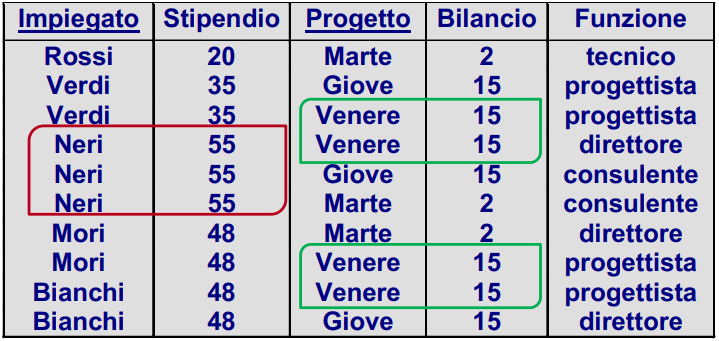
\includegraphics[scale=0.5]{ridondanze.png}
\end{center}
\begin{list}{}{}
	\item \textbf{Ridondanza}: lo stipendio di ogni impiegato è ripetuto in tutte le ennuple relative per ogni progetto a cui partecipa, questo perché \textbf{Stipendio \textit{dipende} solo da Impiegato}
	\item \textbf{Anomalia da aggiornamento}: se lo stipendio varia, è necessario andarne a modificare il valore in diverse ennuple
	\item \textbf{Anomalia da cancellazione}: se un impiegato interrompe la partecipazione a tutti i progetti, dobbiamo cancellare tutte le ennuple in cui appare e così l'impiegato non è più presente nel DB
	\item \textbf{Anomalia da inserimento}: un nuovo impiegato non può essere inserito finché non è assegnato ad un progetto
\end{list}
\subsection{Linee guida per una corretta progettazione}
\paragraph{Semantica degli attributi} Si progetti ogni schema relazionale in modo che \textbf{sia semplice spiegarne il significato}. Non si uniscano attributi provenienti da più tipi di classi e tipi di associazione in un unica relazione.
\paragraph{Ridondanza} Si progettino gli schemi relazionali in modo che nelle relazioni \textbf{non siano presenti anomalie} di inserimento, cancellazione o modifica. Se sono presenti anomalie, le si rilevi chiaramente e ci si assicuri che i programmi che aggiornano il DB operino correttamente.
\paragraph{Valori nulli} Per quanto possibile, \textbf{si eviti di porre attributi i cui valori possono essere frequentemente nulli}. Se è inevitabile, ci si assicuri che essi si presentino solo in casi eccezionali e che non riguardino una maggioranza di tuple nella relazione.
\paragraph{Tuple spurie} Si progettino schemi in modo tale che essi possano essere riuniti tramite join con condizioni di uguaglianza su attributi che sono chiavi primarie o chiavi esterne, in modo da garantire che non vengano generate tuple spurie. \textbf{Non si abbiano relazioni con attributi di accoppiamento diversi dalle combinazioni chiave esterna-chiave primaria}.
\subsection{Dipendenze funzionali}
Per formalizzare la nozione di schema senza anomalie, occorre descrivere formalmente della semantica dei fatti rappresentati in uno schema relazionale.\\
\textbf{Istanza valida di R}: è una \textbf{nozione semantica} che dipende da ciò che sappiamo sul dominio del discorso (non estensionale né deducibile da alcune istanze dello schema $\rightarrow$ confronto con il committente!).\\
Nozione fondamentale: dipendenza funzionale.
\paragraph{Dipendenza funzionale} Data un'istanza valida $r$ su R(T). Siano X e Y due sottoinsiemi non vuoti di T.\\
$\exists$ in $r$ una \textbf{dipendenza funzionale} da X a Y se, $\forall$ coppia di ennuple $t_1$, $t_2$ di $r$ con gli stessi valori su X risulta che $t_1$ e $t_2$ hanno gli stessi valori anche su Y.\\
La dipendenza funzionale da X a Y si denota con X $\rightarrow$ Y.\\\\
Esempio: Persone(CodiceFiscale, Cognome, Nome, DataNascita) ha CodiceFiscale $\rightarrow$ Cognome.\\
Più formalmente:\\\\
Dato uno schema R(T) e X, Y $\subseteq$ T, una \textbf{dipendenza funzionale} (DF) fra gli attributi X e Y è un vincolo su R sulle istanze della relazione espresso nella forma X $\rightarrow$ Y, che significa \textbf{X determina funzionalmente Y} o \textbf{Y è determinato da X}, se $\forall\:\:r$ istanza valida di R $\Rightarrow \forall\:\:t_1,t_2\in r$ si ha $(t_1[X] = t_2[X] \Rightarrow t_1[Y] = t_2[Y])$
\paragraph{Esempio}
\begin{center}
	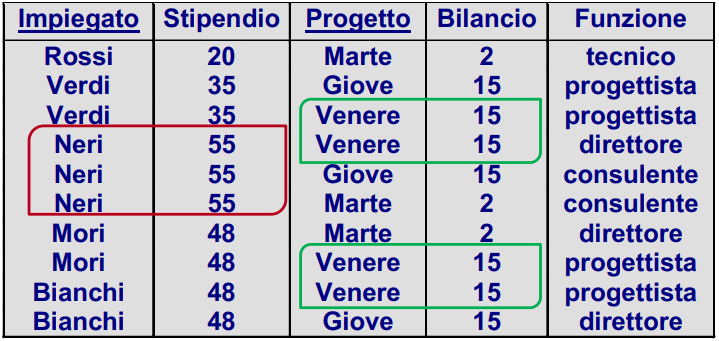
\includegraphics[scale=0.5]{ridondanze.png}
\end{center}
Impiegato $\rightarrow$ Stipendio\\
Progetto $\rightarrow$ Bilancio\\
Impiegato Progetto $\rightarrow$ Funzione\\\\
Le \textbf{dipendenze funzionali sono una proprietà semantica}, cioè \textbf{dipendono dai fatti rappresentati} e non dalla rappresentazione degli attributi negli schemi.
\paragraph{Notazione} Con R$\langle$T, F$\rangle$ si denota uno schema con attributi T e dipendenze funzionali F.\\
Si parla di dipendenza funzionale \textbf{completa} quando X $\rightarrow$ Y e $\forall$ W $\subset$ X non vale W $\rightarrow$ Y.\\
Se X è una superchiave, allora X determina ogni altro attributo della relazione cioè X $\rightarrow$ T. Se X è chiave, allora X $\rightarrow$ T è una dipendenza funzionale completa.
\paragraph{Proprietà} Da un insieme F di dipendenze funzionali, in generale altre dipendenze funzionali sono "implicate" da F. Per esempio (Matricola $\rightarrow$ CodFisc, CodFisc $\rightarrow$ Cognome allora Matricola $\rightarrow$ Cognome)
\begin{list}{}{}
	\item \textbf{Dipendenze implicate}: sia F un insieme di DF sullo schema R, diremo che F \textbf{implica logicamente} X $\rightarrow$ Y (F $\vDash$ X $\rightarrow$ Y) se ogni istanza $r$ di R che soddisfa F soddisfa anche X $\rightarrow$ Y
	\item \textbf{Dipendenze banali}: implicate dal vuoto.\\
	Ad esempio $\{\}\:\vDash\:X \rightarrow Y$
\end{list}
Come derivare le DF implicate logicamente da F? Usando un \textbf{insieme di regole d'inferenza}.
\paragraph{Assiomi di Armstrong} Sono in realtà regole d'inferenza:
\begin{list}{}{}
	\item \textbf{Riflessività R}: Y $\subseteq$ X $\Rightarrow$ X $\rightarrow$ Y
	\item \textbf{Arricchimento A}: X $\rightarrow$ Y $\wedge$ Z $\subseteq$ T $\Rightarrow$ XZ $\rightarrow$ YZ
	\item \textbf{Transitività T}: X $\rightarrow$ Y $\wedge$ Y $\rightarrow$ Z $\Rightarrow$ X $\rightarrow$ Z 
\end{list}
\paragraph{Derivazione} Sia F un insieme di DF. Diremo che \textbf{X $\rightarrow$ Y sia derivabile da F (F $\vdash$ X $\rightarrow$ Y)} se X $\rightarrow$ Y può essere inferito da F usando gli assiomi di Armstrong.\\
Si dimostra che valgono anche le seguenti regole:
\begin{list}{}{}
	\item \textbf{Unione U}: $\{$X $\rightarrow$ Y, X $\rightarrow$ Z$\}\vdash$ X $\rightarrow$ YZ
	\item \textbf{Decomposizione D}: $\{$Z $\subseteq$ Y, X $\rightarrow$ Y$\}\vdash$ X $\rightarrow$ Z
\end{list}
Una derivazione di $f$ da F è una sequenza finita $f_1,\ldots,f_m$ di dipendenze, dove $f_m = f$ e ogni $f_i$ è un elemento di F oppure è ottenuta dalle precedenti dipendenze $f_1\ldots,f_{i-1}$ della derivazione usando una regola d'inferenza.
\paragraph{Correttezza e completezza} Gli assiomi di Armstrong sono corretti e completi. Attraverso essi, si può dimostrare l'equivalenza della nozione di implicazione logica ($\vDash$) e di quella di derivazione ($\vdash$): \textbf{se una dipendenza è derivabile con gli assiomi di Armstrong, allora è anche implicata logicamente} (correttezza) e viceversa \textbf{se una dipendenza è implicata logicamente allora è anche derivabile dagli assiomi} (completezza).\\
Formalmente:
\begin{list}{}{}
	\item $\forall\:f\:\:\:$ F $\vdash\:f\Rightarrow$ F $\vDash\:f$
	\item $\forall\:f\:\:\:$ F $\vDash\:f\Rightarrow$ F $\vdash\:f$
\end{list}
\paragraph{Chiusura di un insieme F} Dato un insieme F di DF, la \textbf{chiusura di F}, denotata con F$^+$, è\\F$^+$ = $\{$X $\rightarrow$ Y $|$ F $\vdash$ X $\rightarrow$ Y$\}$\\
Si presenta spesso il problema di decidere se una dipendenza funzionale appartiene a F$^+$ (\textbf{problema dell'implicazione}). La sua risoluzione con l'algoritmo banale (di generare F$^+$ applicando ad F ripetutamente gli assiomi di Armstrong) ha una \textbf{complessità esponenziale} rispetto al numero di attributi dello schema.\\\\
Dato R$\langle$T, F$\rangle$ e X $\subseteq$ T, la \textbf{chiusura di X rispetto ad F}, denotata con X$_F^+$ (o X$^+$ se F è chiaro dal contesto) è X$_F^+$ = $\{$A$_i\in$ T $|$ F $\vdash$ X $\rightarrow$ A$_i\}$
\paragraph{Problema dell'implicazione} Controllare se una DF V $\rightarrow$ W $\in$ F$^+$.\\
Un algoritmo efficiente per risolverlo senza calcolare F$^+$ parte dal seguente \textbf{teorema}: F $\vdash$ X $\rightarrow$ Y $\Leftrightarrow$ Y $\subseteq$ X$_F^+$
\subparagraph{Idea} Sia X un insieme di attributi e F un insieme di dipendenze. Vogliamo calcolare X$_F^+$.
\begin{enumerate}
	\item Inizializziamo X$^+$ con l'insieme X
	\item Se fra le dipendenze di F c'è una dipendenza Y $\rightarrow$ A con Y $\subseteq$ X$^+$ allora si inserisce A in X$^+$ ossia X$^+$ = X$^+\cup\{$A$\}$
	\item Si ripete 2. fino a quando non ci sono altri attributi da aggiungere a X$^+$
	\item Output X$_F^+$ = X$^+$
\end{enumerate}
\paragraph{Chiavi e attributi primi} Dato lo schema R$\langle$T, F$\rangle$, diremo che un insieme di attributi W $\subseteq$ T è una \textbf{chiave candidata} di R se
\begin{list}{}{}
	\item W \textbf{superchiave}, cioè W $\rightarrow$ T $\in$ F$^+$
	\item V $\subset$ W $\Rightarrow$ V non superchiave, cioè $\forall$ V $\subset$ W, V $\rightarrow$ T $\not\in$ F$^+$
\end{list}
\textbf{Attributo primo}: attributo che appartiene ad almeno una chiave.\\\\
Il problema di trovare tutte le chiavi di una relazione richiede un algoritmo di complessità esponenziale nel caso peggiore.\\
Il problema di controllare se un attributo è primo è NP-Completo.
\pagebreak
\paragraph{Trovare tutte le chiavi} Per trovare tutte le chiavi di R$\langle$T,F$\rangle$ si parte da un insieme di candidati che hanno come base pari all'insieme T meno tutte le parti destre delle dipendenze funzionali in F. Ogni candidato è un sottoinsieme di T rappresentato come X::(Y), che denota dato Y = $\{$A$_1$, \ldots, A$_n\}$ tutti gli insiemi formati da X e da un qualsiasi insieme di attributi A$_i$.\\
Quindi se Base sono gli attributi che non appaiono a destra di nessuna dipendenza, tali attributi devono apparire in ogni chiave per cui inizialmente i candidati sono Base::(T - Base).\\\\
Ogni insieme in X::(Y) è analizzato partendo da X: se è già chiave, allora tutti gli altri insiemi X::(Y) sono scartati, altrimenti si mettono in candidati XA$_1$::(Y-A$_1$), \ldots, XA$_n$::(Y-A$_n$).\\
Se X non contiene chiavi già trovate in precedenza, e X$^+$ = T, allora X è chiave.\\\\
Le chiavi trovate dopo saranno per forza più lunghe, e non potranno essere contenute in una chiave già trovata. Questo si assicura aggiungendo i nuovi candidati in coda alla lista (append), mantenendo quindi la lista dei candidati ordinata per lunghezza.
\subparagraph{Esempio} Con T = $\{$A, B, C, D, E, F$\}$ e F = $\{$C$\rightarrow$D, CF$\rightarrow$B, D$\rightarrow$C, F$\rightarrow$E$\}$\\
La Base è inizializzata quindi con AF attributi, quindi i candidati sono AF::(BCDE).\\
Testando AF, la sua chiusura AF$^+ = \{$A, F, E$\}\neq T$, quindi si prosegue. I candidati sono quindi AF::(BCD) - AF:
\begin{list}{}{}
	\item AFB$^+ = \{$A, F, B, E$\}\neq T$
	\item AFC$^+ = \{$A, F, C, E, D, B$\} = T$ è chiave
	\item AFD$^+ = \{$A, F, D, C, E, B$\} = T$ è chiave
	\item AFBC non si testa, AFC è chiave
	\item AFBD non si testa, AFD è chiave
\end{list}
\section{Copertura Canonica}
\paragraph{Copertura} Due insiemi di dipendenze funzionali F e G sullo schema R sono \textbf{equivalenti} F $\equiv$ G $\Leftrightarrow$ F$^+$ = G$^+$\\
F $\equiv$ G $\Rightarrow$ F è una \textbf{copertura} di G (e G è una copertura di F).
\paragraph{Attributo estraneo} Sia F un insieme di DF.\\
Data una X $\rightarrow$ Y $\in$ F, si dice che X \textbf{contiene un attributo estraneo} A$_i$ $\Leftrightarrow$ (X - $\{$A$_i\}$) $\rightarrow$ Y $\in$ F$^+$, cioè\\F $\vdash$ (X - $\{$A$_i\}$) $\rightarrow$ Y\\
Per verificare se A è estraneo in AX $\rightarrow$ B, calcoliamo X$^+$ e verifichiamo se include B, cioè se basta X a determinare B.
\subparagraph{Un esempio} Consideriamo Orari(CodAula, NomeAula, Piano, Posti, Materia, CDL, Docente, Giorno, Ora)\\
Se vale \begin{list}{}{}
	\item Docente, Giorno, \textit{Ora} $\rightarrow$ CodAula
	\item Docente, Giorno $\rightarrow$ \textit{Ora}
\end{list}
Allora \begin{list}{}{}
	\item Docente, Giorno $\rightarrow$ CodAula
\end{list}
Nella prima dipendenza \textbf{\textit{Ora} è attributo estraneo}.
\paragraph{Dipendenza ridondante} Sia F un insieme di DF.\\
X $\rightarrow$ Y è una \textbf{dipendenza ridondante} $\Leftrightarrow$ (F - $\{$X $\rightarrow$ Y$\}$)$^+$ = F$^+$, cioè F - $\{$X $\rightarrow$ Y$\}$ $\vdash$ X $\rightarrow$ Y\\
Per verificare se X $\rightarrow$ A è ridondante la eliminiamo da F, calcoliamo X$^+$ e verifichiamo se include A, ovvero se con la DF che restano riusciamo ancora a dimostrare che X determina A.
\paragraph{Esempi}
\begin{list}{}{}
	\item F$_1$=$\{$A $\rightarrow$ B, AB $\rightarrow$ C, A $\rightarrow$ C$\}$\\
	Ridondante perché $\{$A $\rightarrow$ B, AB $\rightarrow$ C$\}\Rightarrow$ A $\rightarrow$ C
	\item F$_2$=$\{$A $\rightarrow$ B, AB $\rightarrow$ C$\}$\\
	Non è ridondante, ma B è estraneo perché può essere eliminato dal primo membro della seconda dipendenza
	\item F$_3$=$\{$A $\rightarrow$ B, A $\rightarrow$ C$\}$\\
	Non presenta attributi estranei
\end{list}
\paragraph{Copertura canonica} F è detta copertura canonica $\Leftrightarrow$ \begin{list}{}{}
	\item la parte destra di ogni DF $\in$ F è un attributo
	\item non esistono attributi estranei
	\item nessuna dipendenza è ridondante
\end{list}
\textbf{Teorema}: per ogni insieme F di DF esiste una copertura canonica.\\
La copertura canonica si calcola così:
\begin{list}{}{}
	\item Trasformare le dipendenze nella forma X $\rightarrow$ A\\
Si sostituisce l'insieme dato con quello equivalente che ha tutti i secondi membri costituiti da singoli attributi (\textbf{dipendenze atomiche})
	\item Eliminare gli attributi estranei\\
Per ogni dipendenza si verifica se esistono attributi eliminabili dal primo membro. Cioè $\forall$ X $\rightarrow$ A $\in$ F, verifichiamo se esiste Y $\subseteq$ X $|$ F $\equiv$ F - $\{$X $\rightarrow$ A$\}\cup\{$Y $\rightarrow$ A$\}$
	\item Eliminare le dipendenze ridondanti
\end{list}
\section{Decomposizione di Schemi}
In generale, per eliminare le anomalie da uno schema, occorre decomporlo in schemi più piccoli "equivalenti".
\paragraph{Definizione} Dato uno schema R(T), $\rho$ = $\{$R$_1$(T$_1$),\ldots, R$_k$(T$_k$)$\}$ è una \textbf{decomposizione di R} $\Leftrightarrow$ T$_1$ $\cup$\ldots$\cup$ T$_k$ = T\\
Una decomposizione deve avere due \textbf{proprietà desiderabili}:
\begin{list}{}{}
	\item \textbf{Conservazione dei dati} (nozione semantica)\\
	Una decomposizione $\rho$ = $\{$R$_1$(T$_1$),\ldots, R$_k$(T$_k$)$\}$ di uno schema R(T) \textbf{preserva i dati} $\Leftrightarrow$ $\forall$ istanza \textbf{valida} $r$ di R si ha $r$ = $(\pi_{T_1}r)\vee\ldots\vee(\pi_{T_k}r)$\\
	Dalla definizione di join naturale si ottiene un \textbf{teorema}: se $\rho$ = $\{$R$_1$(T$_1$),\ldots, R$_k$(T$_k$)$\}$ è una decomposizione su R(T) $\Rightarrow$ $\forall$ istanza $r$ di R si ha $r\subseteq(\pi_{T_1}r)\vee\ldots\vee(\pi_{T_k}r)$\\
	Uno schema R(T) si \textbf{decompone senza perdita} negli schemi R$_1$(T$_1$) ed R$_2$(T$_2$) se, per ogni possibile istanza $r$ di R(T), il \textbf{join naturale delle proiezioni di $r$ su T$_1$ ed T$_2$ produce la tabella di partenza} (cioè senza ennuple spurie).\\
	Cioè $\pi_{T_1}(r)\bowtie\pi_{T_2}(r) = r$. La decomposizione senza perdita è garantita se l'insieme degli attributi comuni alle due relazioni (T$_1\cap$T$_2$) è \textbf{chiave per almeno una delle due relazioni decomposte}. Questo perché:
	\begin{list}{}{}
		\item Supponiamo $r$ relazione sugli attributi ABC, consideriamo le sue proiezioni $r_1$ su AB e $r_2$ su AC.
		\item Supponiamo $r$ soddisfi la DF A $\rightarrow$ C, allora \textbf{A è chiave per $r_1$ su AC}, quindi non ci sono in tale proiezione due tuple diverse sui gli stessi valori di A.
		\item Il join costruisce tuple a partire dalle tuple nelle proiezioni.
		\item Sia $t = (a, b, c)$ una tupla del join di $r_1$ ed $r_2$, mostriamo che appartiene ad $r$ (cioè non è spuria): \begin{list}{}{}
			\item $t$ è ottenuta tramite join da $t_1 = (a, b)$ di $r_1$ e $t_2 = (a, c)$ su $r_2$
			\item Allora per definizione di proiezione esistono due tuple in $r$ $t'_1=(a, b, *)$ e $t'_2=(a, *, c)$, dove $*$ sta per valore non noto.
			\item Dato che A $\rightarrow$ C in $r$ allora $\exists$ un solo valore in C associato al valore $a$. Dato che $(a, c)$ compare nella proiezione, questo valore è proprio $c$
			\item Ma allora in $t'_1$ ci deve essere proprio $c$, quindi $(a, b, c) \in r$
		\end{list}
	\end{list}
	\item \textbf{Conservazione delle dipendenze}\\
	Dato lo schema R$\langle$T, F$\rangle$, la decomposizione $\rho = \{$R$_1$,\ldots, R$_n\}$ \textbf{preserva le dipendenze} $\Leftrightarrow$ l'\textbf{unione delle dipendenze in $\pi_{T_i}($F$)$ è una copertura di F}.\\
	Il problema di stabilire se la decomposizione $\rho = \{$R$_1$,\ldots,R$_n\}$ preserva le dipendenze ha complessità di tempo polinomiale. Un \textbf{teorema} importante dice che dato $\rho = \{$R$_i\langle$T$_i$,F$_i\rangle\}$ una decomposizione di R$\langle$T, F$\rangle$ che \textbf{preserva le dipendenze} e tale che T$_j$ \textbf{sia una superchiave di R}, allora $\rho$ \textbf{preserva i dati}.
\end{list}
\paragraph{Qualità} Una decomposizione dovrebbe sempre soddisfare le seguenti \textbf{proprietà}:
\begin{list}{}{}
	\item la \textbf{decomposizione senza perdita}, che garantisce la ricostruzione delle informazioni originarie senza generazione di tuple spurie
	\item la \textbf{conservazione delle dipendenze}, che garantisce il mantenimento dei vincoli d'integrità originari
	\item \textbf{Soddisfacimento della FNBC}: ogni tabella prodotta deve essere in FNBC
\end{list}
\section{Forme Normali}
Una \textbf{forma normale} è una \textbf{proprietà} di un DB relazionale che ne \textbf{garantisce la qualità}, cioè l'assenza di determinati effetti. Quando una relazione non è normalizzata presenta ridondanze e si presta a comportamenti poco desiderabili durante gli aggiornamenti. Ci sono vari tipi di forme normali:
\begin{list}{}{}
	\item \textbf{1FN}: impone una restrizione sul tipo di una relazione, in cui \textbf{ogni attributo ha un tipo elementare}
	\item \textbf{2FN, 3FN e FNBC}: impongono \textbf{restrizioni sulle dipendenze}. FNBC/BCNF (Boyce-Codd) è la più naturale e \textbf{restrittiva}.
\end{list}
\subsection{FNBC} Una relazione $r$ è in FNBC se $\forall$ DF non banale X $\rightarrow$ Y definita su di essa, X \textbf{contiene una chiave K di $r$} (cioè è superchiave).\\
La forma normale non richiede che i concetti in una relazione siano omogenei (solo proprietà direttamente associate alla chiave). L'intuizione è che se esiste in R una dipendenza X $\rightarrow$ A non banale ed X non è chiave, allora X modella l'identità di un'entità diversa da quelle modellate dall'intera R.
\paragraph{Definizione} R$\langle$T,F$\rangle$ è in BCNF $\Leftrightarrow$ $\forall$ X $\rightarrow$ A $\in$ F$^+$, con A $\not\in$ X (non banale), X è una superchiave
\subparagraph{Teorema} R$\langle$T,F$\rangle$ è in BCNF $\Leftrightarrow$ $\forall$ X $\rightarrow$ A $\in$ F non banale, X è una superchiave
\paragraph{L'algoritmo di analisi} R$\langle$T,F$\rangle$ è decomposta in R$_1$(X, Y) e R$_2$(X, Z) e su di esse si ripete il procedimento, esponenziale.
\paragraph{} A vole la decomposizione per raggiungere la BCNF può risultare difficile o impossibile, ed occorre quindi ricorrere ad una forma normale indebolita.
\subsection{3FN}
Una relazione $r$ è in 3NF se $\forall$ DF non banale X $\rightarrow$ Y definita su $r$, è verificata almeno una delle seguenti condizioni:
\begin{list}{}{}
	\item X contiene una chiave K di $r$ (come nella BCNF)
	\item ogni attributo in Y è contenuto in almeno una chiave K di $r$
\end{list}
Meno restrittiva della FNBC: tollera alcune ridondanze e certifica meno la qualità dello schema ottenuto, ma è \textbf{sempre ottenibile} qualunque sia lo schema di partenza. Basta usare l'algoritmo di normalizzazione in TFN.
\subsection{Algoritmo di Sintesi (versione base)}
\paragraph{Input} Insieme R di attributi e insieme F di dipendenze su R
\paragraph{Output} Decomposizione $\rho = \{$S$_i\}_{i=1\ldots n}$ di R tale che preservi i dati e le dipendenze ed ogni S$_i$ sia in 3NF rispetto alle proiezioni di F su S$_i$.
\begin{enumerate}
	\item Trova una copertura canonica G di F e poni $\rho = \{\}$
	\item Sostituisci in G ogni insieme X $\rightarrow$ A$_1$, \ldots, X $\rightarrow$ A$_h$ di dipendenze con lo stesso determinante con la dipendenza X $\rightarrow$ A$_1$\ldots A$_h$
	\item Per ogni dipendenza X $\rightarrow$ Y in G metti uno schema con attributi XY in $\rho$
	\item Elimina da $\rho$ ogni schema che sia contenuto in un altro schema di $\rho$
	\item Se la decomposizione non contiene alcuno schema i cui attributi costituiscano una superchiave per R, aggiungi ad essa lo schema con attributi W, con W una chiave di R.
\end{enumerate}
\chapter{DBMS}
Un DBMS deve gestire grandi quantità di dati persistenti e condivisi. La gestione richiede \textbf{particolare attenzione ai problemi di efficienza}, come l'ottimizzazione delle richieste ma non solo.\\
La \textbf{persistenza} e la \textbf{condivisione} richiedono che un DBMS fornisca dei \textbf{meccanismi per garantire l'affidabilità dei dati} (\textbf{fault tolerance}), per il \textbf{controllo degli accessi} e per il \textbf{controllo della concorrenza}. Diverse altre funzionalità vengono messe a disposizione per motivi di efficacia, ovvero per semplificare la descrizione dei dati, lo sviluppo delle applicazioni, l'amministrazione del DB\ldots
\paragraph{Condivisione dei dati} La \textbf{gestione integrata} e la \textbf{condivisione dei dati} permettono di evitare le ripetizioni (ridondanza dovuta a copie multiple dello stesso dato) e quindi di \textbf{evitare un inutile spreco di risorse} (memoria).\\
Inoltre, la \textbf{ridondanza può dare luogo a problemi di inconsistenza} delle copie e comporta la necessità di propagare le modifiche, con un ulteriore spreco di risorse (CPU e rete).
\paragraph{Modello dei dati} Dal punto di vista utente, un DB è visto come una collezione di dati che modellano una certa porzione della realtà di interesse.\\
L'\textbf{astrazione logica} con cui i dati vengono resi disponibili all'utente \textbf{definisce un modello dei dati}. Più precisamente: \textbf{un modello dei dati è una collezione di concetti che vengono utilizzati per descrivere i dati, le loro associazioni/relazioni ed i vincoli che questi devono rispettare}.\\
Un \textbf{ruolo di primaria importanza} nella definizione di un modello dei dati è svolto dai \textbf{meccanismi che possono essere usati per strutturare i dati} (tipo i costruttori di tipo in un linguaggio di programmazione). Per esempio, ci sono modelli in cui i dati sono descritti solo sotto forma di albero (modello \textbf{gerarchico}), di grafi (modello \textbf{reticolare}), di oggetti complessi (modello \textbf{a oggetti}), di relazioni (modello \textbf{relazionale}).
\paragraph{Indipendenza fisica e logica} Tra gli obiettivi di un DBMS, vi sono quelli di fornire caratteristiche di
\begin{list}{}{}
	\item \textbf{Indipendenza fisica} dei dati: dipende da considerazioni legate all'efficienza delle organizzazioni adottate. \textbf{La riorganizzazione fisica dei dati non deve comportare effetti collaterali sui programmi applicativi}.
	\item \textbf{Indipendenza logica}: permette di \textbf{accedere ai dati logici indipendentemente dalla loro rappresentazione fisica}.
\end{list}
\pagebreak
\section{Architettura semplificata di un DBMS}
\begin{center}
	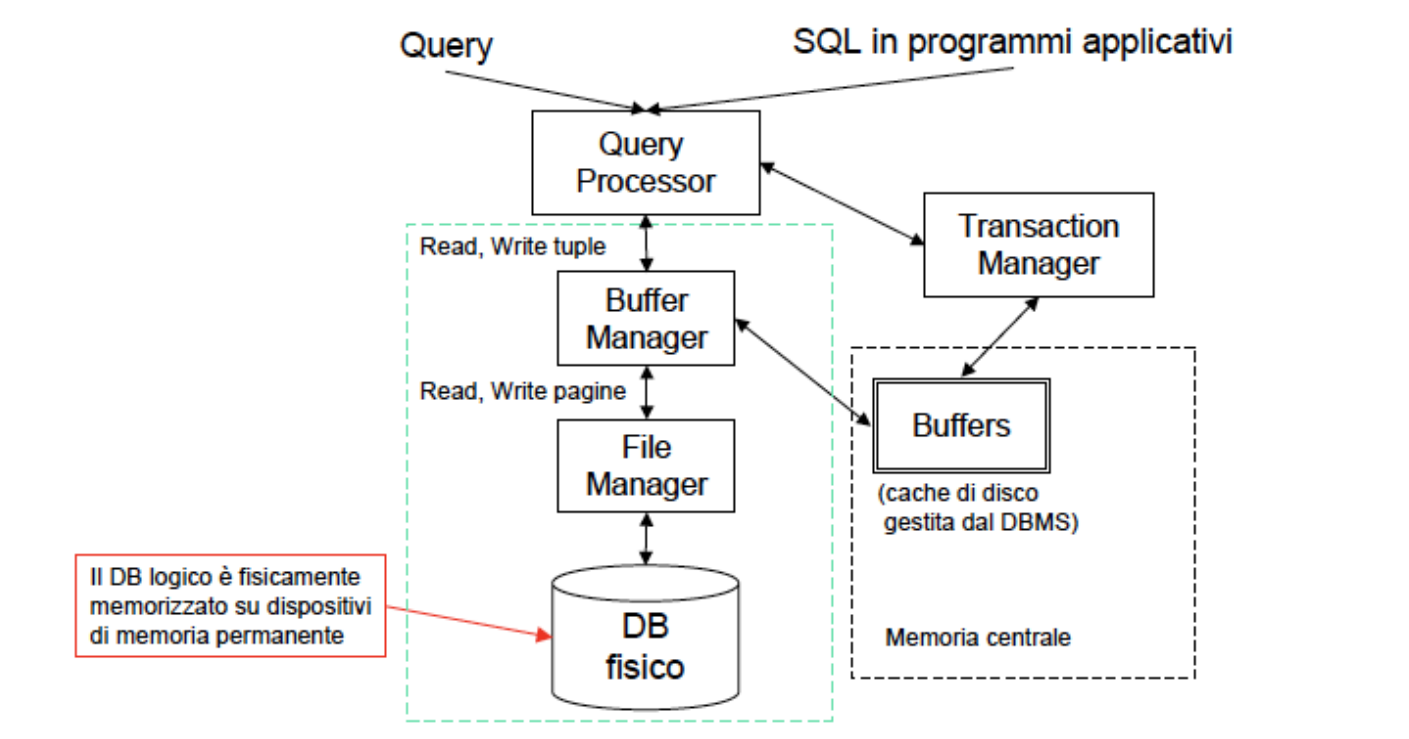
\includegraphics[scale=0.45]{dbmsstrutt.png}\\
	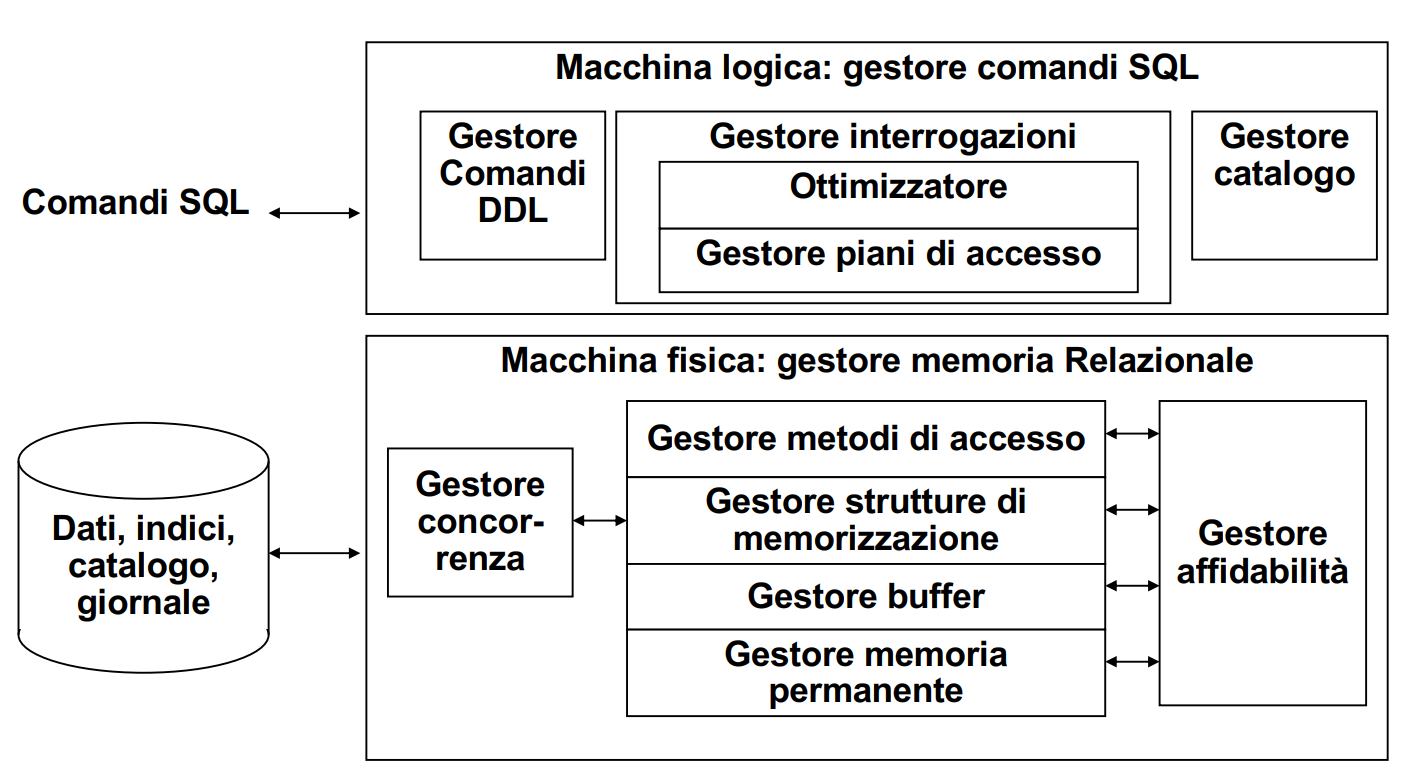
\includegraphics[scale=0.45]{dbmslogfis.png}
\end{center}
\paragraph{Gerarchia di memoria} La memoria in un sistema di calcolo è organizzata in una gerarchia: al livello più alto ci sono memorie di piccola dimensione, molto veloci e costose, mentre più si scende più la dimensione aumenta e si riducono velocità e costi.\\
Le prestazioni si misurano in termini di tempo di accesso
\begin{center}
\textsl{Tempo di accesso} = \textsl{latenza} + $\frac{\textsl{dimensione dati da trasferire}}{\textsl{velocità di trasferimento}}$
\end{center}
A causa delle dimensioni, un DB solitamente risiede sui dischi. I dati devono essere trasferiti in memoria centrale per essere elaborati dal DBMS: il \textbf{trasferimento non avviene a singole tuple ma a blocchi}, anche detti pagine.\\\\
\pagebreak
Spesso le operazioni di I/O costituiscono il \textbf{collo di bottiglia di un sistema}, quindi è necessario\\\textbf{ottimizzare l'implementazione fisica del DB} attraverso:
\begin{list}{}{}
	\item Organizzazione efficiente delle tuple su disco
	\item Strutture di accesso efficienti
	\item Gestione efficiente dei buffer in memoria
	\item Strategie di esecuzione efficienti per le query
\end{list}
\subsection{Gestore di memoria permanente} Fornisce un'astrazione della memoria permanente in termini di insiemi di file logici, di pagine fisiche e di blocchi, nascondendo le caratteristiche dei dischi e del sistema operativo.
\subsection{Gestore del buffer} Si preoccupa del trasferimento delle pagine tra la memoria temporanea e la memoria permanente, offrendo agli altri livelli una visione della memoria permanente come un insieme di pagine utilizzabili in memoria temporanea, astraendo da quando esse vengano trasferite dalla memoria permanente al buffer e viceversa.\\
Nei DBMS, la LRU per rimpiazzare le pagine non è sempre una buona scelta. Per alcune query, il "pattern di accesso" ai dati è noto e quindi può essere utilizzato per operare scelte più accurate, in grado di migliorare anche di molto le prestazioni.
\subsection{Gestore strutture di memorizzazione}
\paragraph{Tipi di organizzazione}\begin{list}{}{}
	\item \textbf{Seriali/Sequenziali}\\
	Organizzazione \textbf{seriale} (\textbf{heap file}): i dati sono memorizzati in modo \textbf{disordinato} uno dopo l'altro. Semplice, a basso costo di memoria, poco efficiente quindi va bene per pochi dati. Organizzazione standard di ogni DBMS.\\
	Organizzazione \textbf{sequenziale}: i dati sono \textbf{ordinati} sul valore di uno o più attributi, così da avere ricerche più veloci, ma le nuove inserzioni fanno perdere l'ordinamento. Costo di ricerca di $\log_2 b_i + 1$ accessi per ogni blocco, se ogni file contiene $b_i$ blocchi dato che la ricerca binaria richiede $\log_2 b$ accessi.-
	\item \textbf{Per chiave}\\
	Obiettivo: noto il valore di una chiave, trovare il record di una tabella con qualche accesso al disco (idealmente uno solo).\\
	Alternative: metodo procedurale (hash) o tabellare (indice), organizzazione statica o dinamica.
	\item \textbf{Per attributi non chiave}
\end{list}
\paragraph{Parametri che caratterizzano un'organizzazione}\begin{list}{}{}
	\item Occupazione di memoria
	\item Costo delle operazioni di: ricerca, modifica, inserzione, cancellazione
\end{list}
\paragraph{Ordinamento di archivi} Ordinare gli archivi è importante per eseguire alcune operazioni relazionali (JOIN, SELECT DISTINCT, GROUP BY) e per avere risultati ordinati dalle interrogazioni (ORDER BY).
\subparagraph{Algoritmo} L'algoritmo utilizzato costa N$\cdot\log$(N): è lo Z-way merge sort (merge sort a Z vie).\\
Supponiamo di dover ordinare un input che consiste in un file di NP pagine e di avere a disposizione solo NB $<$ NP buffer in memoria centrale. L'algoritmo opera in due fasi:
\begin{list}{}{}
	\item \textbf{Sort interno}: si leggono una alla volta le pagine del file. I \textbf{record di ogni pagina sono ordinati facendo uso di un algoritmo di sort interno} (es: quicksort). \textbf{Ogni pagina così ordinata}, detta anche \textbf{run}, \textbf{viene scritta su disco} in un file \textbf{temporaneo}.
	\item \textbf{Merge}: operando \textbf{uno o più passi di fusione} le \textbf{run vengono fuse fino a produrne una sola}.
\end{list}
Per la \textbf{complessità}, consideriamo il solo numero di operazioni I/O al caso base Z = 2 e NB = 3. Si osserva che:
\begin{list}{}{}
	\item Nella fase di sort interno si leggono e riscrivono NP pagine
	\item Ad ogni passo di merge si leggono e riscrivono NP pagine\\
	Il numero di passi di fusione è pari a $\lceil\log_2$NP$\rceil$, in quanto ad ogni passo il numero di run si dimezza.
	\item Il \textbf{costo complessivo} è pertanto $2\cdot$NP$\cdot(\lceil\log_2$NP$\rceil+1)$
\end{list}
Al caso generale, possiamo osservare che nel passo di sort interno si possono ordinare NB pagine alla volta invece che una sola, il che abbassa il costo a $2\cdot$NP$\cdot(\lceil\log_2$(NP/NB)$\rceil+1)$\\\\
Oltre che per ordinare le tuple, il sort può essere usato per le query dove compare DISTINCT, per eliminare i duplicati, oppure anche per le query contenenti GROUP BY.
\section{Piani di accesso}
\begin{enumerate}
	\item Analisi lessicale e sintattica del comando SQL Q\\
	\texttt{SQLCommand parseTree = Parser.parseStatement(Q);}
	\item Analisi semantica del comando\\
	\texttt{Type type = parseTree.check();}
	\item Ottimizzazione dell'interrogazione\\
	\texttt{Value pianoDiAccesso = parseTree.Optimize();}
	\item Esecuzione del piano di accesso
\end{enumerate}
\begin{multicols}{2}
	\begin{center}
		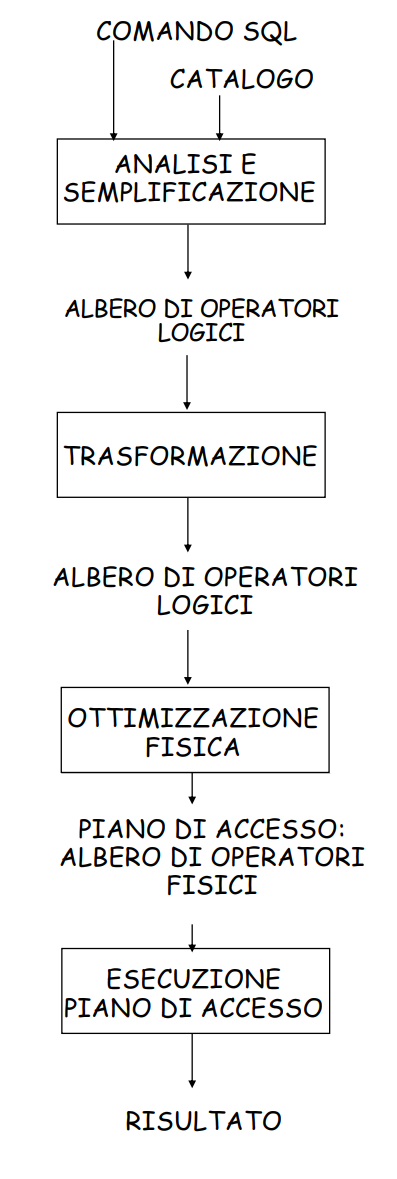
\includegraphics[scale=0.5]{ottimizz.png}
	\end{center}
	\columnbreak
	\textbf{Analisi e semplificazione}: verifica la correttezza del comando, normalizzazione e semplificazione della condizione.\\
	\textbf{Piano di accesso}: \textbf{scelta} dell'algoritmo per eseguire ogni operatore: \textbf{Ideale}, trovare il piano migliore, ed \textbf{Euristica}, evitare i piani peggiori.
	\begin{lstlisting}
	SELECT	Nome
	FROM	Studenti S, Esami E
	WHERE	S.Matricola = E.Matricola
		AND Provincia = "PI"
		AND VOTO > 25
	\end{lstlisting}
	\begin{center}
		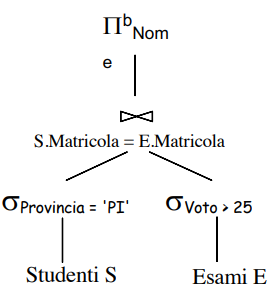
\includegraphics[scale=0.5]{ottimizzazese.png}\\
		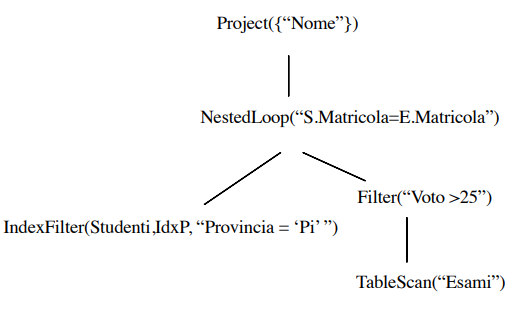
\includegraphics[scale=0.5]{ottimizzazese2.png}
	\end{center}
	Le foglie sono le tabelle ed i nodi interni specificano le modalità con cui gli accessi alle tabelle e le operazioni relazionali sono effettuate.
\end{multicols}
\paragraph{Realizzazione degli operatori relazionali} Si considerano gli operatori di: proiezione, selezione, raggruppamento, join.\\
Un \textbf{operatore può essere realizzato con algoritmi diversi}, \textbf{codificati in opportuni operatori fisici}.
\paragraph{Operatori fisici} Gli algoritmi per realizzare gli operatori relazionali si codificano in opportuni operatori fisici. Ad esempio, \texttt{TableScan(R)} è l'operatore fisico per la scansione di R.\\
Ogni operatore fisico è un \textbf{iteratore}, cioè un \textbf{oggetto con metodi} \texttt{open}, \texttt{next}, \texttt{isDone}, \texttt{reset} e \texttt{close}, realizzati usando gli operatori della macchina fisica e con \texttt{next} che ritorna un record.\\
Prenderemo come esempio gli operatori fisici del sistema JRS, usandoli per descrivere un algoritmo che esegue un'interrogazione SQL.
\begin{list}{}{}
	\item \texttt{open}: inizializza lo stato dell'operatore,  alloca buffer per gli input e l’output, richiama ricorsivamente open sugli operatori figli; viene anche usato per passare argomenti (ad es. la condizione che un operatore \texttt{Filter} deve applicare)
	\item \texttt{next}: usato per richiedere un’altra tupla del risultato dell’operatore. L’implementazione di questo metodo include \texttt{next} sugli operatori figli e codice specifico dell’operatore
	\item \texttt{close}: usato per terminare l’esecuzione dell’operatore, con conseguente rilascio delle risorse ad esso allocate
	\item \texttt{isDone}: indica se vi sono ancora valori da leggere, in genera è booleano.
\end{list}
Il \textbf{piano di accesso} quindi, cioè l'algoritmo che viene usato per eseguire un'interrogazione usando gli operatori fisici disponibili, è rappresentato da un albero del tipo
\begin{center}
	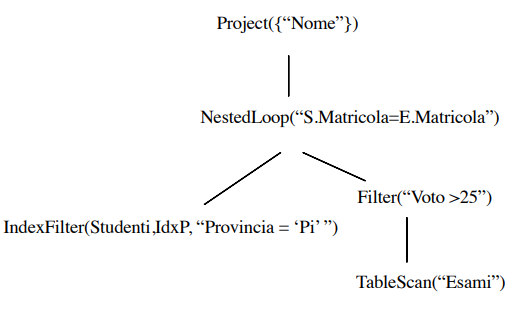
\includegraphics[scale=0.75]{ottimizzazese2.png}
\end{center}
\begin{tabular}{c | l}
\textbf{Operatore logico} & \textbf{Operatore fisico}\\
\hline
R & \makecell[l]{\texttt{TableScan(R)} per la scansione di R\\\texttt{IndexScan(R, Idx)} per la scansione di R con l'indice Idx\\\texttt{SortScan(R, \{A$_i$\})} per la scansione di R ordinata sugli \{A$_i$\}}\\
\hline
\makecell{$\pi^b_{\{A_i\}}$\\$\pi_{\{A_i\}}$} & \makecell[l]{\texttt{Project(O, \{A$_i$\})} per la proiezione dei record i O senza l'eliminazione dei duplicati\\\texttt{Distinct(O)} per eliminare i duplicati dei record ordinati da O}\\
\hline
$\sigma_\psi$ & \makecell[l]{\texttt{Filter(O, $\psi$)} per la restrizione senza indici dei record di O\\\texttt{IndexFilter(R, Idx, $\psi$)} per la restrizione con indice dei record di R}\\
\hline
$\tau_{\{A_i\}}$ & \texttt{Sort(O, \{A$_i$\})} per ordinare i record di O sugli \{A$_i$\}, per valori crescenti\\
\hline
$_{\{A_i\}}\gamma_{\{f_i\}}$ & \makecell[l]{\texttt{GroupBy(O, \{A$_i$\}, \{f$_i$\})} per raggruppare i record di O sugli \{A$_i$\} usando le\\funzioni di aggregazione in \{f$_i$\}.\\
Nell'insieme \{f$_i$\} vi sono le funzioni di aggregazione presenti nella SELECT e nella HAVING.\\L'operatore ritorna record con attributi gli \{A$_i$\} e le funzioni in \{f$_i$\}\\I record di O sono ordinati sugli \{A$_i$\}}\\
\hline
$\bowtie_{\psi_j}$ & \makecell[l]{\texttt{NestedLoop(O$_E$, O$_I$, $\psi_j$)} per la join con il \textbf{nested loop} e $\psi_j$ condizione di join\\\texttt{PageNestedLoop(O$_E$, O$_I$, $\psi_j$)} per la join con il \textbf{page nested loop}\\\texttt{IndexNestedLoop(O$_E$, O$_I$, $\psi_j$)} per la join con l'\textbf{index nested loop}. L'operando interno O$_I$\\è un \texttt{IndexFilter(R, Idx, $\psi_j$)} oppure \texttt{Filter(O, $\psi'$)} con O un \texttt{IndexFilter(R, Idx, $\psi_j$)}.\\Per ogni record $r$ di O$_E$, la condizione $\psi_j$ dell'\texttt{IndexFilter} è quella di giunzione con\\gli attributi di O$_E$ sostituiti dai valori in $r$.\\\texttt{SortMerge(O$_E$, O$_I$, $\psi_j$)} per la giunzione con il \textbf{sort-merge}, con i record di O$_E$ e O$_I$ ordinati\\ sugli attributi di giunzione}
\end{tabular}
\pagebreak
\paragraph{Indice} Struttura dati con informazioni sulla posizione di memorizzazione delle tuple in base al valore del campo chiave. Solo per file sequenziali (ordinati)
\begin{list}{}{}
	\item \textbf{Indice primario} quando la chiave di ordinamento del file sequenziale coincide con la chiave di ricerca dell'indice.\\
	$\langle$K($i$), RID($i$)$\rangle$: il primo campo è lo stesso tipo del campo chiave di ordinamento (PK), il secondo è un puntatore ad un blocco del disco.
	\item \textbf{Indice secondario} se la chiave di ordinamento e la chiave di ricerca sono diverse.\\
	Definito su un campo non chiave: il primo campo è dello stesso tipo del campo che non viene usato per ordinare il file ed è chiamato campo di indicizzazione, il secondo è un puntatore ad un blocco del disco.
\end{list}
Può essere definito su un insieme di attributi, in questo caso contiene un record per ogni combinazione di valori assunti dagli attributi e può essere usato per rispondere efficientemente ad interrogazioni che specifichino un valore per ciascun attributo.
\section{Transazioni}
Durante le transazioni vengono interessati il \textbf{gestore della concorrenza} e il \textbf{gestore dell'affidabilità}.\\
Le \textbf{transazioni} rappresentano le \textbf{unità di lavoro elementare} (le insiemi di istruzioni SQL) che \textbf{modificano il contenuto di un DB}. Sintatticamente, una transazione è contornata dai comandi \texttt{BEGIN TRANSACTION} e \texttt{END TRANSACTION}, e all'interno possono comparire i comandi di \texttt{COMMIT WORK} e \texttt{ROLLBACK WORK}.
\begin{lstlisting}
BEGIN TRANSACTION
UPDATE SalariImpiegati
SET Conto = Conto - 10
WHERE (CodiceImpiegato = 123)
IF (Conto > 10) COMMIT WORK
ELSE ROLLBACK WORK
\end{lstlisting}
\paragraph{ACID} Le transazioni devono godere delle proprietà ACID:
\begin{list}{}{}
	\item \textbf{Atomicità}: la transazione deve essere eseguita con la regola \textbf{tutto o niente}.
	\item \textbf{Consistenza}: la transazione deve \textbf{lasciare il DB in uno stato consistente}, quindi \textbf{eventuali vincoli d'integrità non devono essere violati}.
	\item \textbf{Isolamento}: ogni transazione deve essere \textbf{eseguita in maniera indipendente dalle altre}
	\item Persistenza (\textbf{Durability}): l'\textbf{effetto di una transazione che ha fatto \texttt{COMMIT WORK} non deve essere perso}.
\end{list}
\paragraph{Funzioni del DBMS in breve}
\begin{center}
	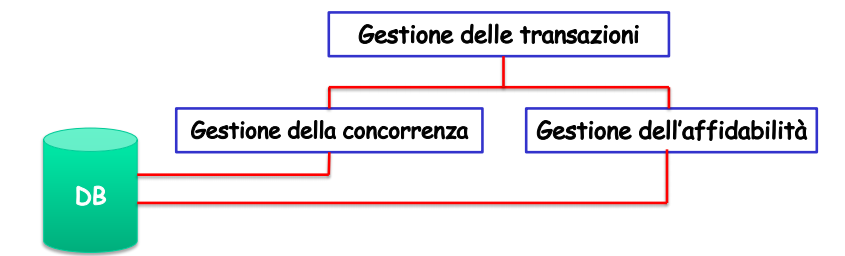
\includegraphics[scale=0.75]{funzdbbreve.png}
\end{center}
\begin{list}{}{}
	\item \textbf{Gestione dei dati}: cura la memorizzazione permanente dei dati ed il loro accesso
	\item \textbf{Gestione del buffer}: cura il trasferimento dei dati da memoria di massa a memoria centrale, e il caching dei dati in memoria centrale
	\item \textbf{Ottimizzazione delle interrogazioni}: seleziona il piano di accesso di costo ottimo con cui valutare ciascuna interrogazione
\end{list}
\pagebreak
\section{Gestione dell'affidabilità}
Una transazione è un'unità logica di elaborazione che corrisponde ad una serie di operazioni fisiche elementari (letture e scrittura) sul DB. Una \textbf{funzionalità essenziale} di un DBMS è la \textbf{protezione dei dati da malfuzionamenti e interferenze} dovute all'accesso contemporaneo ai dati da parte di più utenti.\\
Per il \textbf{programmatore}, una \textbf{transazione} è un \textbf{programma sequenziale che il sistema deve eseguire garantendo}:
\begin{list}{}{}
	\item \textbf{Atomicità}: le transazioni che terminano prematuramente (\textbf{aborted transactions}) sono \textbf{trattate dal sistema come se non fossero mai iniziate}, pertanto eventuali effetti sul DB sono annullati.
	\item \textbf{Persistenza}: le \textbf{modifiche} sulla base di dati di una transazione terminata normalmente sono permanenti, cioè \textbf{non sono alterabili} da eventuali malfunzionamenti.
	\item \textbf{Serializzabilità}: nel caso di \textbf{esecuzioni concorrenti} di più transazioni, l'\textbf{effetto complessivo è quello di un'esecuzione seriale}.
\end{list}
Per aumentare l'efficiente prestazionale, tutti i DBMS utilizano un buffer temporaneo di informazioni in memoria principale, il quale viene periodicamente scritto su memoria secondaria.
\begin{center}
	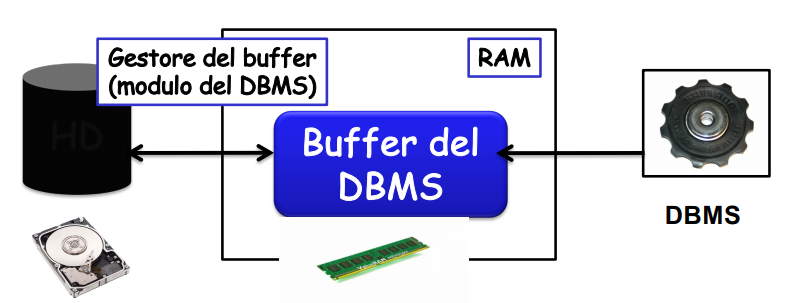
\includegraphics[scale=0.5]{dbmsbuffer.png}
\end{center}
\paragraph{Transazione per il DBMS} Una transazione può eseguire molte operazioni sui dati recuperati da un DB, ma al DBMS interessano solo quelle di lettura o scrittura del DB indicate con $r_i[x]$ e $w_i[x]$.\\
Un dato letto o scritto può essere un record, un campo di un record o una pagina. Per semplicità, supponiamo che sia una pagina.\\\\
Un'operazione di lettura $r_i[x]$ comporta la lettura di una pagina nel buffer, se non già presente.\\
Un'operazione di scrittura $w_i[x]$ comporta l'\textbf{eventuale lettura nel buffer di una pagina e la sua modifica nel buffer, ma non necessariamente la sua scrittura in memoria permanente}. Per questa ragione, in caso di malfunzionamento, si potrebbe perdere l'effetto dell'operazione.
\paragraph{Malfunzionamenti}
\begin{list}{}{}
	\item \textbf{Fallimenti di transazioni}: non comportano la perdita di dati in memoria temporanea né persistente (es: violazione di vincoli, violazione di protezione, stallo\ldots)
	\item \textbf{Fallimenti di sistema}: comportano la perdita di dati in memoria temporanea ma non in memoria persistente (es: comportamento anomalo del sistema, blackout, guasti hardware\ldots)
	\item \textbf{Disastri}: comportano la perdita di dati in memoria permanente (es: danneggiamento di una periferica)
\end{list}
Il \textbf{gestore dell'affidabilità verifica che siano garantite le proprietà di atomicità e persistenza delle transazioni}. Responsabile di:\begin{list}{}{}
	\item implementare i comandi di \texttt{BEGIN TRANSACTION}, \texttt{COMMIT} e \texttt{ROLLBACK}
	\item ripristinare il sistema dopo malfunzionamenti software (\textbf{ripresa a caldo})
	\item ripristinare il sistema dopo malfunzionamento hardware (\textbf{ripresa a freddo})
\end{list}
\paragraph{Primitive undo e redo} Partiamo da convenzioni notazionali: data una transazione T, indicheremo con B(T), C(T) e A(T) rispettivamente i record di begin, commit e abort relativi a T, e con U(T, O, BS, AS), I(T, O, AS) e D(T, O, BS) rispettivamente i record di update, insert e delete su un oggetto O dove BS è before state e AS è after state.\\
\textbf{I record del log} associati ad una transazione \textbf{consentono di disfare e rifare le corrispondenti azioni} sul DB:
\begin{list}{}{}
	\item \textbf{Primitive di undo}: per \textbf{disfare} un'azione su un oggetto O è sufficiente ricopiare il O il valore BS (l'insert viene disfatto cancellando l'O inserito)
	\item \textbf{Primitive di redo}: per \textbf{rifare} un'azione su un oggetto O è sufficiente ricopiare in O il valore AS (il delete viene rifatto cancellando l'O eliminato)
\end{list}
\paragraph{File di log} Il controllore dell'affidabilità usa \textbf{un log, dove sono indicate tutte le operazioni svolte dal DBMS}. Il file si presenta come una sequenza di record di due tipi:
\begin{list}{}{}
	\item \textbf{Record di transizione}: tengono traccia delle operazioni svolte da ciascuna transizione sul DBMS. Per ogni transazione, un record di begin (B), insert (I), delete (D) e update (U) e un record di commit (C) o di abort(A)
	\item \textbf{Record di sistema}: tengono traccia delle operazioni di sistema (dump, checkpoint).\\
	\textbf{Dump} produce una \textbf{copia completa} del DB, effettuata in mutua esclusione con tutte le altre transazioni quando il sistema non è operativo. La copia viene memorizzata in memoria stabile (backup). Al termine del dump, viene scritto nel log un record di dump che segnala l'avvenuta esecuzione dell'operazione in un dato istante. Il sistema quindi riprende il funzionamento normale.\\
	\textbf{Checkpoint}, punto di allineamento: si scrive la marca CKP sul log per indicare che tutte le operazioni che la precedono sono state effettivamente effettuate sul DB. Un modo semplice:
	\begin{list}{}{}
		\item Si sospende l'attivazione di nuove transazioni
		\item si completano le precedente e si allinea il DB (ovvero si scrivono su disco le pagine "sporche" del buffer)
		\item si scrive la marca CKP nel log
		\item si riprende l'esecuzione
	\end{list}
	Per non bloccare le transazioni, si può scrivere un BeginCKP e un EndCKP: tra di loro si copia su disco in parallelo alle normali operazioni, e le transazioni loggate nel mezzo possono essere o non essere state copiate su disco.
\end{list}
Contenuto:
\begin{list}{}{}
	\item \texttt{(T, begin)}
	\item Per ogni operazione di modifica:
	\begin{list}{}{}
		\item la transazione responsabile
		\item il tipo di ogni operazione eseguita
		\item la nuova e vecchia versione del dato modificato\\
		\texttt{(T, write, address, oldV, newV)}
	\end{list}
	\item \texttt{(T, commit)} o \texttt{(T, abort)}
\end{list}
\paragraph{Regole di scrittura}
\begin{list}{}{}
	\item \textbf{Write Ahead Log} (WAL): la parte BS di ogni record viene \textbf{scritta prima che la corrispondente operazione venga effettuata nella base di dati}.
	\item \textbf{Commit Precedence}: la parte AS di ogni record di log viene \textbf{scritta prima di effettuare il commit della transazione}.
\end{list}
\paragraph{Ripresa}\begin{list}{}{}
	\item Fallimenti di transazioni: si scrive \texttt{(T, abort)} su log e si fa l'undo
	\item Fallimenti di sistema: DB ripristinato con il comando di \texttt{Restart} (ripartenza di emergenza), a partire dallo stato al punto di allineamento, procedendo così: le \textbf{T non terminate vengono disfatte}, e le \textbf{T terminate devono essere rifatte}.
	\item Disastri: si riporta in linea la copia più recente del DB e la si aggiorna rifacendo le modifiche delle T terminate normalmente (ripartenza a freddo)
\end{list}
Per la \textbf{ripresa a caldo} ci sono quattro fasi
\begin{enumerate}
	\item Trovare l'ultimo checkpoint (percorrendo log a ritroso)
	\item Costruire gli insiemi UNDO e REDO delle transazioni da disfare e rifare
	\item Ripercorrere il log all'indietro, fino alla più vecchia delle transazioni in UNDO e REDO, disfacendo tutte le azioni delle transazioni in UNDO
	\item Ripercorrere il log in avanti, rifacendo tutte le azioni delle transazioni REDO
\end{enumerate}
Nella \textbf{ripresa a freddo} si risponde ad un guasto che provoca il deterioramento del DB:
\begin{list}{}{}
	\item Si ripristinano i dati dal backup
	\item Si eseguono le operazioni registrate sul giornale fino all'istante del guasto
	\item Si esegue una ripresa a caldo.
\end{list}
\paragraph{Ricapitolando} Gli algoritmi si differenziano a seconda del modo in cui si trattano le scritture sul DB e la terminazione delle transazioni: disfare-rifare, disfare-non rifare, non disfare-rifare, non disfare-non rifare.\\
Per ipotesi, le scritture sul log sono riportate subito nella memoria permanente.
\section{Gestione della concorrenza}
\paragraph{Serializzazione} Uno schedule S si dice \textbf{seriale se le azioni di ciascuna transazione appaiono in sequenza} senza essere inframezzate da azioni di altre transazioni.\\
S = \{T$_1$, \ldots, T$_n$\}\\
Lo \textbf{schedule seriale è ottenibile se}:
\begin{list}{}{}
	\item Le \textbf{transazioni sono eseguite una alla volta} (scenario irrealistico)
	\item Le \textbf{transazioni sono completamente indipendenti} l'una dall'altra (improbabile)
\end{list}
\subparagraph{ACID} Proprietà di isolamento delle transazioni.\\
Il DBMS transazionale gestisce questi problemi garantendo la \textbf{proprietà di isolamento}: questa proprietà \textbf{garantisce che la transazione sia eseguita come se non ci fosse concorrenza}. Viene \textbf{assicurata facendo in modo che ciascun insieme di transazioni concorrenti sottoposte sia serializzabile}.
\paragraph{Problematica} In un sistema reale, le \textbf{transazioni vengono eseguite in concorrenza} per questioni di efficienza e scalabilità. Tuttavia, l'esecuzione concorrente determina un \textbf{insieme di problematiche} che devono essere gestite. Un esempio:
\begin{list}{}{}
	\item \texttt{T1 = Read(x); x = x + 1; Write(x); COMMIT WORK}
	\item \texttt{T2 = Read(x); x = x + 1; Write(x); COMMIT WORK}
	\item Se \texttt{x} = 3, allora al termine delle due transazioni \texttt{x} = 5 (\textbf{esecuzione sequenziale}).\\
	Nel caso di esecuzione concorrente invece si possono verificare tanti casi (ipotizzando \texttt{x} = 3 inizialmente):
	\begin{list}{}{}
		\item \textbf{Perdita di aggiornamento}
		\begin{center}
			\begin{tabular}{l | l}
				T1 & T2\\
				\hline
				\texttt{Read(x)} & \\
				\texttt{x = x + 1} & \\
				& \texttt{Read(x)}\\
				& \texttt{x = x + 1}\\
				& \texttt{Write(x)}\\
				& \texttt{COMMIT WORK}\\
				& \textit{Scrive 4} \\
				\texttt{Write(x)} & \\
				\texttt{COMMIT WORK} & \\
				\textit{Scrive 4} &
			\end{tabular}
		\end{center}
		\item \textbf{Lettura sporca/impropria}\\
		\texttt{T1 = Read(x); x = x + 1; Write(x); ROLLBACK WORK}\\
		\texttt{T2 = Read(x); COMMIT WORK}
		\begin{center}
			\begin{tabular}{l | l}
				T1 & T2\\
				\hline
				\texttt{Read(x)} & \\
				\texttt{x = x + 1} & \\
				\texttt{Write(x)} & \\
				& \texttt{Read(x)}\\
				& \texttt{COMMIT WORK}\\
				& \textit{Legge 4} \\
				\texttt{ROLLBACK WORK} &
			\end{tabular}
		\end{center}
		\item \textbf{Letture inconsistenti}/\textbf{non riproducibili}\\
		\texttt{T1 = Read(x); Read(x); COMMIT WORK}\\
		\texttt{T2 = Read(x);  x = x + 1; Write(x); COMMIT WORK}
		\begin{center}
			\begin{tabular}{l | l}
				T1 & T2\\
				\hline
				\texttt{Read(x)} & \\
				\textit{Legge 3} & \\
				& \texttt{Read(x)}\\
				& \texttt{x = x + 1}\\
				& \texttt{Write(x)}\\
				& \texttt{COMMIT WORK}\\
				\texttt{Read(x)} & \\
				\texttt{COMMIT WORK} & \\
				\textit{Legge 4}
			\end{tabular}
		\end{center}
	\end{list}
	Quindi l'\textbf{esecuzione concorrente di transazioni è essenziale per un buon funzionamento del DBMS}: deve garantire che l'esecuzione concorrente di transazioni avvenga senza interferenze in caso di accessi agli stessi dati.
\end{list}
\paragraph{Serialità} Un'esecuzione di un insieme di transazioni \{T$_1$, \ldots, T$_n$\} si dice \textbf{seriale} se $\forall$ coppia di transazioni T$_i$, T$_j$, tutte le operazioni di T$_i$ vengono eseguite prime di qualsiasi operazione di T$_j$ o viceversa.
\paragraph{Serializzabilità} Un'esecuzione di un insieme di transazioni si dice \textbf{serializzabile} se produce lo stesso effetto sulla base di dati di quello ottenibile eseguendo serialmente, in un qualche ordine, le sole transazioni terminate normalmente.
\paragraph{Controllo della concorrenza} Nella pratica i DBMS implementano tecniche di controllo di concorrenza che garantiscono direttamente la serializzabilità delle transazioni concorrenti. Tali tecniche si dividono in due classi principali:
\begin{list}{}{}
	\item \textbf{Protocolli ottimistici}: \textbf{permettono l'esecuzione sovrapposta e non sincronizzata di transazioni} ed effettuano un \textbf{controllo sui possibili conflitti generati solo dopo il commit}.\\
	Ogni transazione effettua liberamente le proprie operazioni sugli oggetti del DB secondo l'ordine temporale con cui le operazioni sono generate.\\
	Al \textbf{commit}, viene \textbf{effettuato un controllo} per stabilire se sono stati riscontrati eventuali conflitti e, in caso, viene \textbf{effettuato il rollback delle azioni} delle transazioni e la relativa riesecuzione. In generale, un protocollo ottimistico è \textbf{basato su 3 fasi}:
	\begin{list}{}{}
		\item Fase di \textbf{lettura}: ogni transazione legge i valori degli oggetti del DB su cui deve operare e li memorizza in variabili locali (copie), dove sono effettuati gli eventuali aggiornamenti.
		\item Fase di \textbf{validazione}: vengono effettuati dei controlli sulla serializzabilità nel caso che gli aggiornamenti locali delle transazioni dovessero essere propagati sul DB
		\item Fase di \textbf{scrittura}: gli aggiornamenti delle transazioni che hanno superato la fase di validazione sono propagati definitivamente sugli oggetti del DB.
	\end{list}
	\item \textbf{Protocolli pessimistici}/conservativi: \textbf{tendono a ritardare l'esecuzione di transazioni che potrebbero generare conflitti}, e quindi anomalie, rispetto alla transazioni concorrente. Cercano di \textbf{prevenire}, e sono quelli usati nella pratica. Si dividono in due classi principali:
	\begin{list}{}{}
		\item Metodi \textbf{basati su lock}\\
		I DBMS commerciali usano il meccanismo dei \textbf{lock}: per poter effettuare una qualsiasi operazione di lettura/scrittura su una risorsa (tabella o valore di una cella) è \textbf{necessario aver precedentemente acquisito il controllo, cioè il lock, sulla risorsa stessa}.
		\begin{list}{}{}
			\item \textbf{Lock in lettura}, per l'\textbf{accesso esclusivo}
			\item \textbf{Lock in scrittura}, per la \textbf{mutua esclusione}
		\end{list}
		Ci possono essere lock a livello di riga, tabella o pagina (\textbf{multi granularità}), oltre che in lettura o scrittua (\textbf{multi modalità}).\\
		Quando una risorsa è bloccata, le transazioni che ne richiedono l'accesso vengono messe in coda d'attesa: è un meccanismo efficace ma incide sulle prestazioni.
		Un esempio di richiesta e rilascio del lock:
		\begin{multicols}{2}
			Codice utente
			\begin{lstlisting}
Transazione T0:
	R(x)
	W(y)
			\end{lstlisting}
			\columnbreak
			Codice con lock
			\begin{lstlisting}
Transazione T0:
	lockR(x)
	R(x)
	unlockR(x)
	lockW(y)
	W(y)
	unlockW(y)
			\end{lstlisting}
		\end{multicols}
		Il gestore della concorrenza del DBMS ha quindi il compito di stabilire l'ordine con cui vengono eseguite le singole operazioni per rendere serializzabile l'esecuzione di un insieme di transazioni.\\
		\textbf{Definizione}: il protocollo di blocco a due fasi ristretto (\textbf{Strict Two Phase Locking}, 2PL) è definito dalle seguenti regole:
		\begin{list}{}{}
			\item Ogni transazione prima di effettuare un'operazione acquisisce il lock corrispondente.
			\item Transazioni diverse non ottengono lock in conflitto
			\item I lock si rilasciano al commit $\rightarrow$ \textbf{problema}: deadlock. Esempio:
			\begin{multicols}{2}
			\texttt{T1 = R(x); W(y); COMMIT WORK}\\
			\texttt{T2 = R(y); W(x); COMMIT WORK}
			\columnbreak
			
			\begin{tabular}{l | l}
				T1 & T2 \\
				\hline
				\texttt{lockR(x)} & \\
				& \texttt{lockR(y)} \\
				\texttt{R(x)} & \\
				& \texttt{R(y)} \\
				\texttt{lockW(y)} & \\
				& \texttt{lockW(y)} \\
				\textit{Stallo} & \textit{Stallo}
			\end{tabular}
			\end{multicols}
			Si può gestire con \textbf{tre tecniche}:
			\begin{enumerate}
				\item Uso dei \textbf{timeout}: \textbf{ogni operazione di una transazione ha un timeout} entro il quale deve essere completata, pena l'\textbf{abort dell'intera transazione}.\\
\texttt{T1 = lockR(x, 4000); R(x); lockW(y, 2000); W(y); COMMIT WORK; unlock(x); unlock(y);}				
				\item \textbf{Deadlock avoidance}: prevenire le configurazioni che potrebbero portare a deadlock: \textbf{lock/unlock di tutte le risorse contemporaneamente} oppure \textbf{utilizzo di timestamp/classi di priorità tra transazioni} (ma può portare a starvation)
				\item \textbf{Deadlock detection}: usare \textbf{algoritmi per identificare i deadlock} e prevedere meccanismi di recovery. Ad esempio, il grafo delle richieste/risorse e abort delle transazioni coinvolte nel cicli.
			\end{enumerate}
		\end{list}
		\item Metodi \textbf{basati su timestamp}\\
		Ad ogni transazione si associa un \textbf{timestamp} che rappresenta il momento di inizio della transazione. Ogni transazione \textbf{non può leggere o scrivere un dato scritto da una transazione con timestamp maggiore} né \textbf{può scrivere su un dato già letto da una transazione con timestamp maggiore}.
	\end{list}
\end{list}
\pagebreak
\paragraph{Livelli di isolamento/consistenza per ogni transazione}
\begin{list}{}{}
	\item \textbf{SERIALIZABLE} assicura che:
	\begin{list}{}{}
		\item La transazione T legge solo i cambiamenti fatti da transazioni che hanno fatto commit
		\item Nessun valore letto o scritto da T verrà cambiato da altre transazioni finché T non è conclusa
		\item Se T legge un insieme di valori acceduti secondo qualche condizione di ricerca, l'insieme non viene modificato da altre transazioni finché T non è conclusa
	\end{list}
	\item \textbf{REPEATABLE READ} assicura che:
	\begin{list}{}{}
		\item La transazione T legge solo i cambiamenti fatti da transazioni che hanno fatto commit
		\item Nessun valore letto o scritto da T verrà cambiato da altre transazioni finché T non è conclusa
	\end{list}
	\item \textbf{READ COMMITED} assicura che:
	\begin{list}{}{}
		\item La transazione T legge solo i cambiamenti fatti da transazioni che hanno fatto commit
		\item T non vede nessun cambiamento eventualmente effettuato da transazioni concorrenti non concluse tra i valori letti all'inizio di T
	\end{list}
	\item \textbf{READ UNCOMMITTED}\\
	A questo livello di isolamento una transazione T può leggere modifiche fatte ad un oggetto da una transazione in esecuzione. Ovviamente l'oggetto può essere cambiato mentre T è in esecuzione: per questo \textbf{T è soggetta a eventi fantasma}.
\end{list}
\end{document}